\chapter{Case studies}
\label{chp:case_studies}
%-------------------------------------------------------------------------------

\noindent{\LARGE\textbf{Case study 1}}
%===============================================================================
\section{A mechanistic emulator: fitting the \emph{weir equation}}
\label{sec:mechanistic_emulator}
%===============================================================================

%:::::::::::::::::::::::::::::::::::::::::::::::::::::::::::::::::::::::::::::::
%  * present it as a didactic example
%  * use it to compare GP (prior knowledge) with e.g. deep neural networks: how many points can we have?
%  * mention grid convergence study (results go in the Appendix)
%  * mention problem with FullSWOF boundary conditions
%  * define well results and methodology
%  * such an emulator can be improved -> modified to compute slope in order to have a given mu value
%  * state all of the goals of the CS: learn weir eq. from simulation, apply curve fitting, get a feeling for simulation accuracy
%:::::::::::::::::::::::::::::::::::::::::::::::::::::::::::::::::::::::::::::::

As a first case study to apply the acquired knowledge, it was decided to build an utterly mechanistic emulator.
The main goal of this case study is to try to fit the \emph{weir equation} to simulated data instead of to experimental data.
Here we essentially rediscover the way science has always been done: by observing, measuring and trying to discover mathematical relationships.
The most significant difference is the fact that the experimental set-up is completely computer built.\\

The \emph{weir equation} is a partially theoretical equation that provides an estimate of the discharge $Q$ over a weir as a function of the water depth above the weir itself ($h_w$).
The equation can be derived from the Bernoulli equation under certain assumptions \autocite{bos_discharge_1989} and can be found in many different forms.
The form used here is the one proposed by \emph{Francis} \autocite{walcott_weir_1907}:

\begin{equation}\label{eq:weir_eq}
  Q = \textcolor{red}{C} \cdot L \cdot h_w^{\textcolor{red}{a}}\, , \quad \mbox{usu. } \textcolor{red}{a = 3/2}
\end{equation}

\noindent Where the empirical coefficient $C$ corrects for the assumption of absence of viscous effects and uniform velocity distribution, $L$ is the length of the weir (perpendicular to the channel) and $h_w$ is the water height above the weir.

In addition to the parametric model (\textit{weir equation}) two non-parametric local techniques, namely \emph{linear interpolation} and \emph{cubic spline interpolation}, were used to intrapolate between the simulated data points.\\


%-------------------------------------------------------------------------------
\subsection{Brief experiment description}\label{sec:cs1_brief_description}
%-------------------------------------------------------------------------------

For this experiment, simulations were run in a flat rectangular channel.
A weir with a trapezoidal cross section is located at the channel half-length.
As initial condition the upstream side of the weir was filled with water up to the weir crest.
At the domain top boundary a constant inflow discharge was set, while at the bottom boundary water could freely outflow.
As the simulation runs, the inflow water flows down the channel, overflows the weir and leaves the domain through the lower boundary (see Fig.~\ref{fig:channel}).
After some time the simulation reaches the \emph{steady-state} conditions: inflow, discharge over the weir and outflow have the same magnitude and the water height above the weir has stabilized.
At this point the value $h_w$ was extracted and was paired with the discharge value $Q$ generating it.
\num{25} experiments were conducted with $Q$ linearly spaced in the range \SIrange{0.1}{10}{\cubic\meter\per\second}.
All simulated pairs $(Q, h_w)$ constitute an \emph{inputs-output} sets to which the weir equation was fitted.\\

In order to ensure the convergence of the simulator solution, and therefore the quality of the experimental results, a \emph{grid convergence study} was performed prior to the experiment.
For this, the simulation with the highest discharge was repeated with successive grid refinements.
The value of the variable of interest, water height, was then compared between the different simulations to find at which grid resolution the solution stabilizes.


%-------------------------------------------------------------------------------
\subsection{Material and methods}
%-------------------------------------------------------------------------------
%...............................................................................
\subsubsection{Generating the topography}
%...............................................................................
The topography used for running the simulations was generated in \citetalias{octave_community_gnu_2018} and represents a flat channel of \SI{40}{\meter} length with a weir placed at its midpoint, at \SI{20}{\meter} distance from the top boundary.
The channel cross section is a rectangle of \SI{4}{\meter} width and the weir has a trapezoidal shape.
Fig.~\ref{fig:weir_scheme} shows the geometry of the channel.
The weir has a crest width of \SI{2}{\meter} and therefore belongs to the \emph{broad-crested} class. The $C$ coefficient for broad-crested weirs with vertical walls and \SI{2}{\meter} crest width varies between \num{1.36} and \num{1.53}, depending on the water height $h_w$ \autocite{brown_urban_2009}.
We therefore expect a value close to this for our experiment.

\begin{figure}[h]
  \centering
  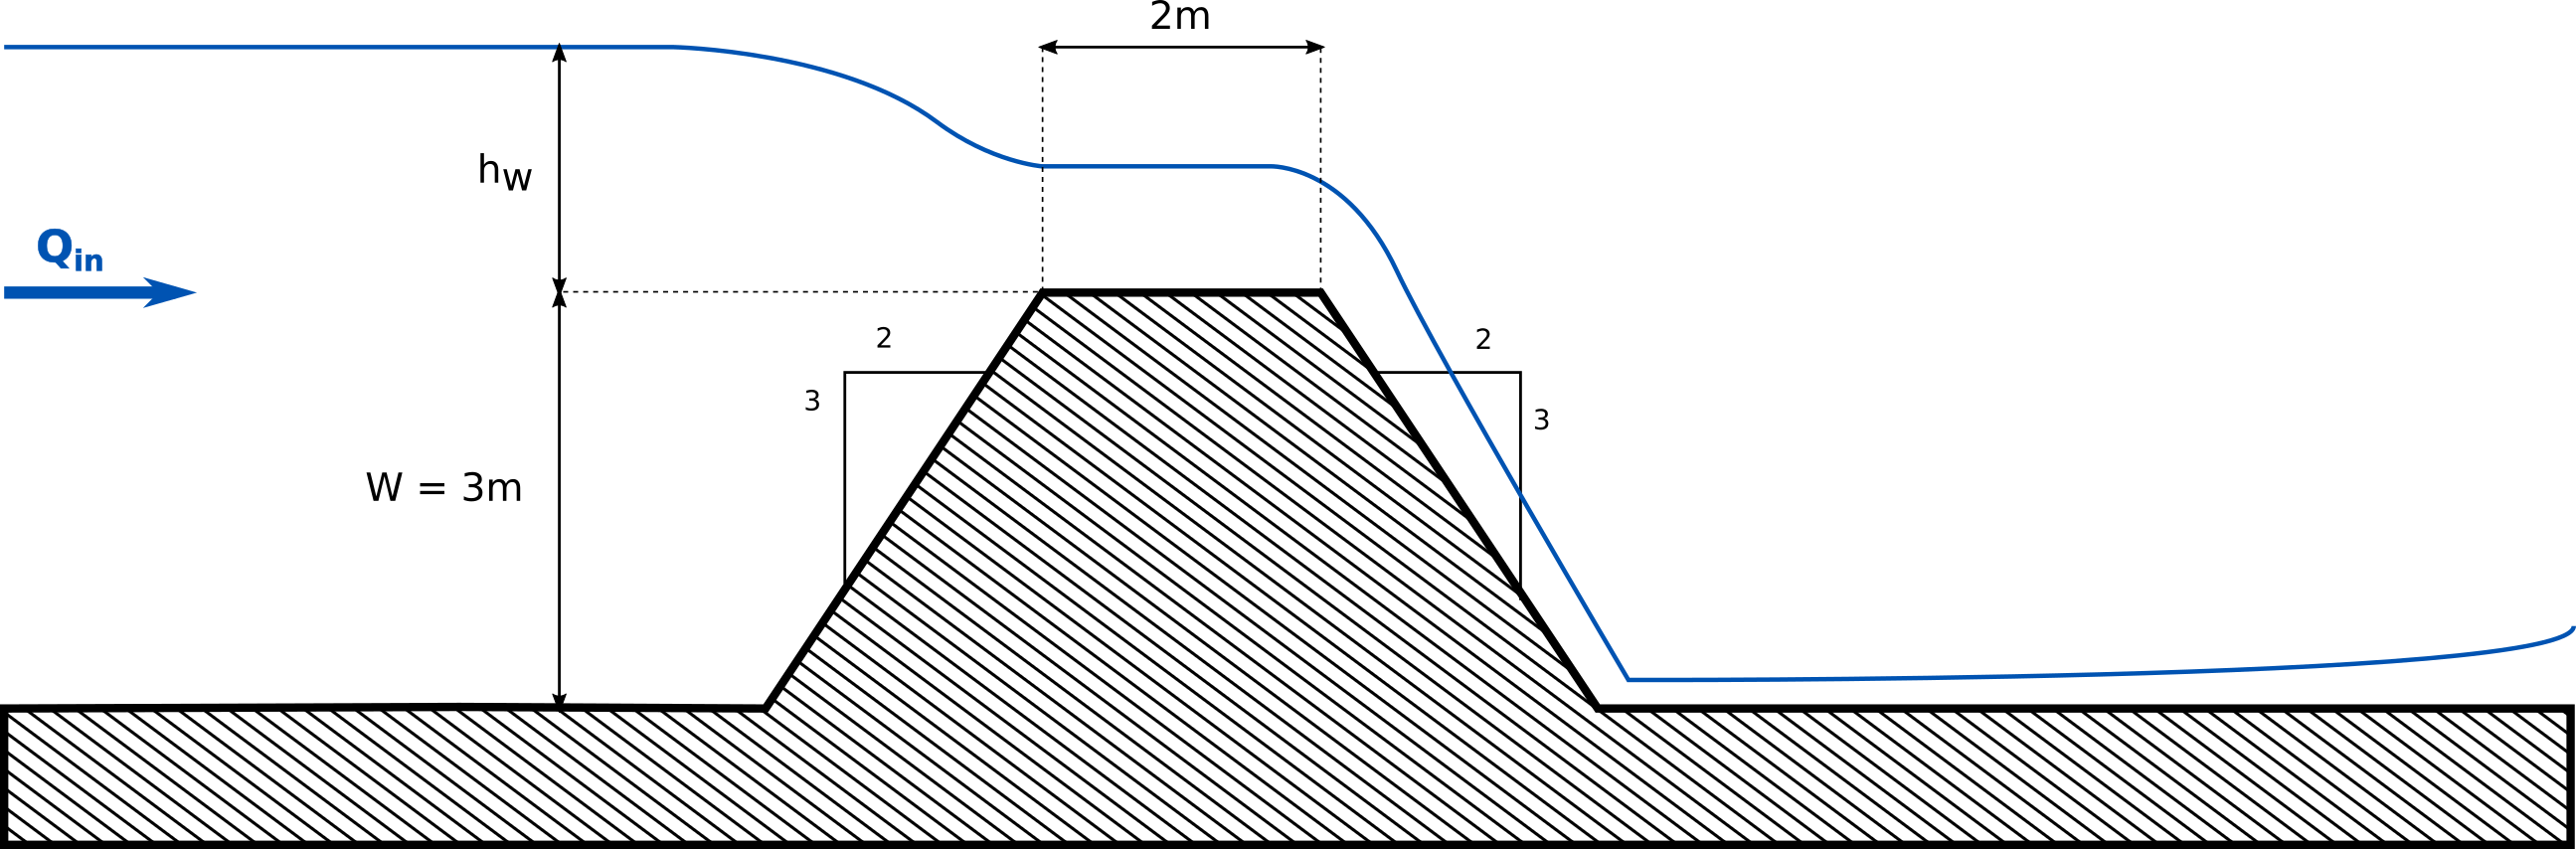
\includegraphics[width=0.8\textwidth]{Figures/weir_scheme.png}
  \caption{Geometry of the weir used for the experiments.}
  \label{fig:weir_scheme}
\end{figure}

%...............................................................................
\subsubsection{Setting-up the simulations}
%...............................................................................
After generating the topography to be used for the experiment the simulation parameters were defined.

The simulation was done with no rain and no infiltration.
This way, water just enters the system through the top boundary and leaves it through the bottom one.
For this a \emph{Neumann} boundary condition was chosen at the bottom, while an \emph{imposed discharge} boundary condition was set at the inflow boundary.
This boundary condition needs two values to be specified: the magnitude of the inflow and an imposed water height, which is used under supercritical flow conditions.
The \num{25} inflow discharges used were obtained with the following \citetalias{octave_community_gnu_2018} code:\\

\inputminted[
  fontsize=\footnotesize,
  firstline=4,
  lastline=5,
  numbersep=2pt,
  gobble=0,
  frame=none,
  bgcolor=light-gray,
  framesep=10mm
]{octave}{code.m}\\

\noindent where, by definition within \citetalias{delestre_fullswof:_2017}, the minus sign indicates that water steadily \emph{enters the domain}.
The imposed height was set to \SI{3}{\m}, corresponding to the weir height.

The channel topography presents no banks.
Wall boundary conditions were set for the lateral boundaries in order to produce the rectangular cross section.
The wall boundaries extend infinitely high, preventing the water from overflowing.
Simulations were run for $t_{max} = \SI{200}{\s}$ and \num{200} intermediate states were saved, giving a time resolution of the simulation output of \SI{1}{\s}.
For the channel a uniform Manning roughness coefficient of \SI{0.03}{\s\per\m\tothe{1/3}} was used.

Since infiltration was not active for the simulations, all of the parameters relative to the soil model did not have to be set.

The number of cells in x, and in y direction were defined according to the grid convergence study explained here below.


%...............................................................................
\subsubsection{Conducting the grid convergence study}
%...............................................................................
The chosen grid resolution influences accuracy of simulation results as well as simulation runtime.
In order to find the appropriate grid resolution, a grid convergence study was performed.
Successive refinements were tested in order to find out at which resolution the solution converges.
A criterion has to be established, in order to decide when the solution has satisfactorily converged.
If the Grid Convergence Index (GCI) is used, then a GCI lower than \SI{5}{\percent} for the last refinement is usually taken as a criterion \autocite{ali_grid_2009}.

For the mesh study \num{7} simulations were run by varying the grid resolution ($Nx$, $Ny$) only.
Topography and parameters used are those mentioned in the two preceding sections.
Squared cells were used and the inflow discharge was set to the highest discharge value of the experiment, namely \SI{10}{\cubic\meter\per\second}.
This discharge is the one generating the highest flow velocities.
If convergence under these conditions is reached, then convergence for lower discharges is also assured.
Tab.~\ref{tab:mesh_study} summarizes the simulations' main characteristics.

\begin{table}[h]
  \centering
  \caption{Summary of simulations runtime, grid resolution and other related parameters for the mesh convergence study.}
  \label{tab:mesh_study}
  \begin{tabular}{crrcccccr}
    \toprule
    \# & \multicolumn{1}{c}{Nx} & \multicolumn{1}{c}{Ny} & \multicolumn{1}{c}{Lx $[\si{\m}]$} & \multicolumn{1}{c}{Ly $[\si{\m}]$} & \multicolumn{1}{c}{dx $[\si{\m}]$} & \multicolumn{1}{c}{dy $[\si{\m}]$} & \multicolumn{1}{c}{Q $[\si{\cubic\m\per\s}]$} & \multicolumn{1}{c}{runtime $[\si{\s}]$} \\
    \midrule
    1  & 2             & 20            & 4               & 40          & 2.00        & 2.00        & 10                      & 0.00 \\
    2  & 4             & 40            & 4               & 40          & 1.00        & 1.00        & 10                      & 0.07 \\
    3  & 8             & 80            & 4               & 40          & 0.50        & 0.50        & 10                      & 0.60 \\
    4  & 20            & 200           & 4               & 40          & 0.20        & 0.20        & 10                      & 9.00 \\
    5  & 40            & 400           & 4               & 40          & 0.10        & 0.10        & 10                      & 69.60 \\
    6  & 80            & 800           & 4               & 40          & 0.05        & 0.05        & 10                      & 537.72 \\
    7  & 100           & 1000          & 4               & 40          & 0.04        & 0.04        & 10                      & 1048.40 \\
    \bottomrule
  \end{tabular}
\end{table}

Fig.~\ref{fig:water_profiles} shows the free surface profiles of the \num{7} simulations at steady-state conditions along the channel axis.
It can be noticed that for $Ny =$ \numlist{20;40;80} the water depth is visibly higher than for further refinements, and its shape quite varying.
This means that the solution has not converged yet.
Results for $Ny =$ \numlist{400;800;1000} are very close, since the lines are almost overlapping.
$Ny =$ \num{200} shows a similar profile shape, but the height is still diverging significantly from the successive refinements.
To better observe the variations between the different refinements, the $h$ value convergence at the weir crest was studied.

\begin{figure}[h]
  \centering
  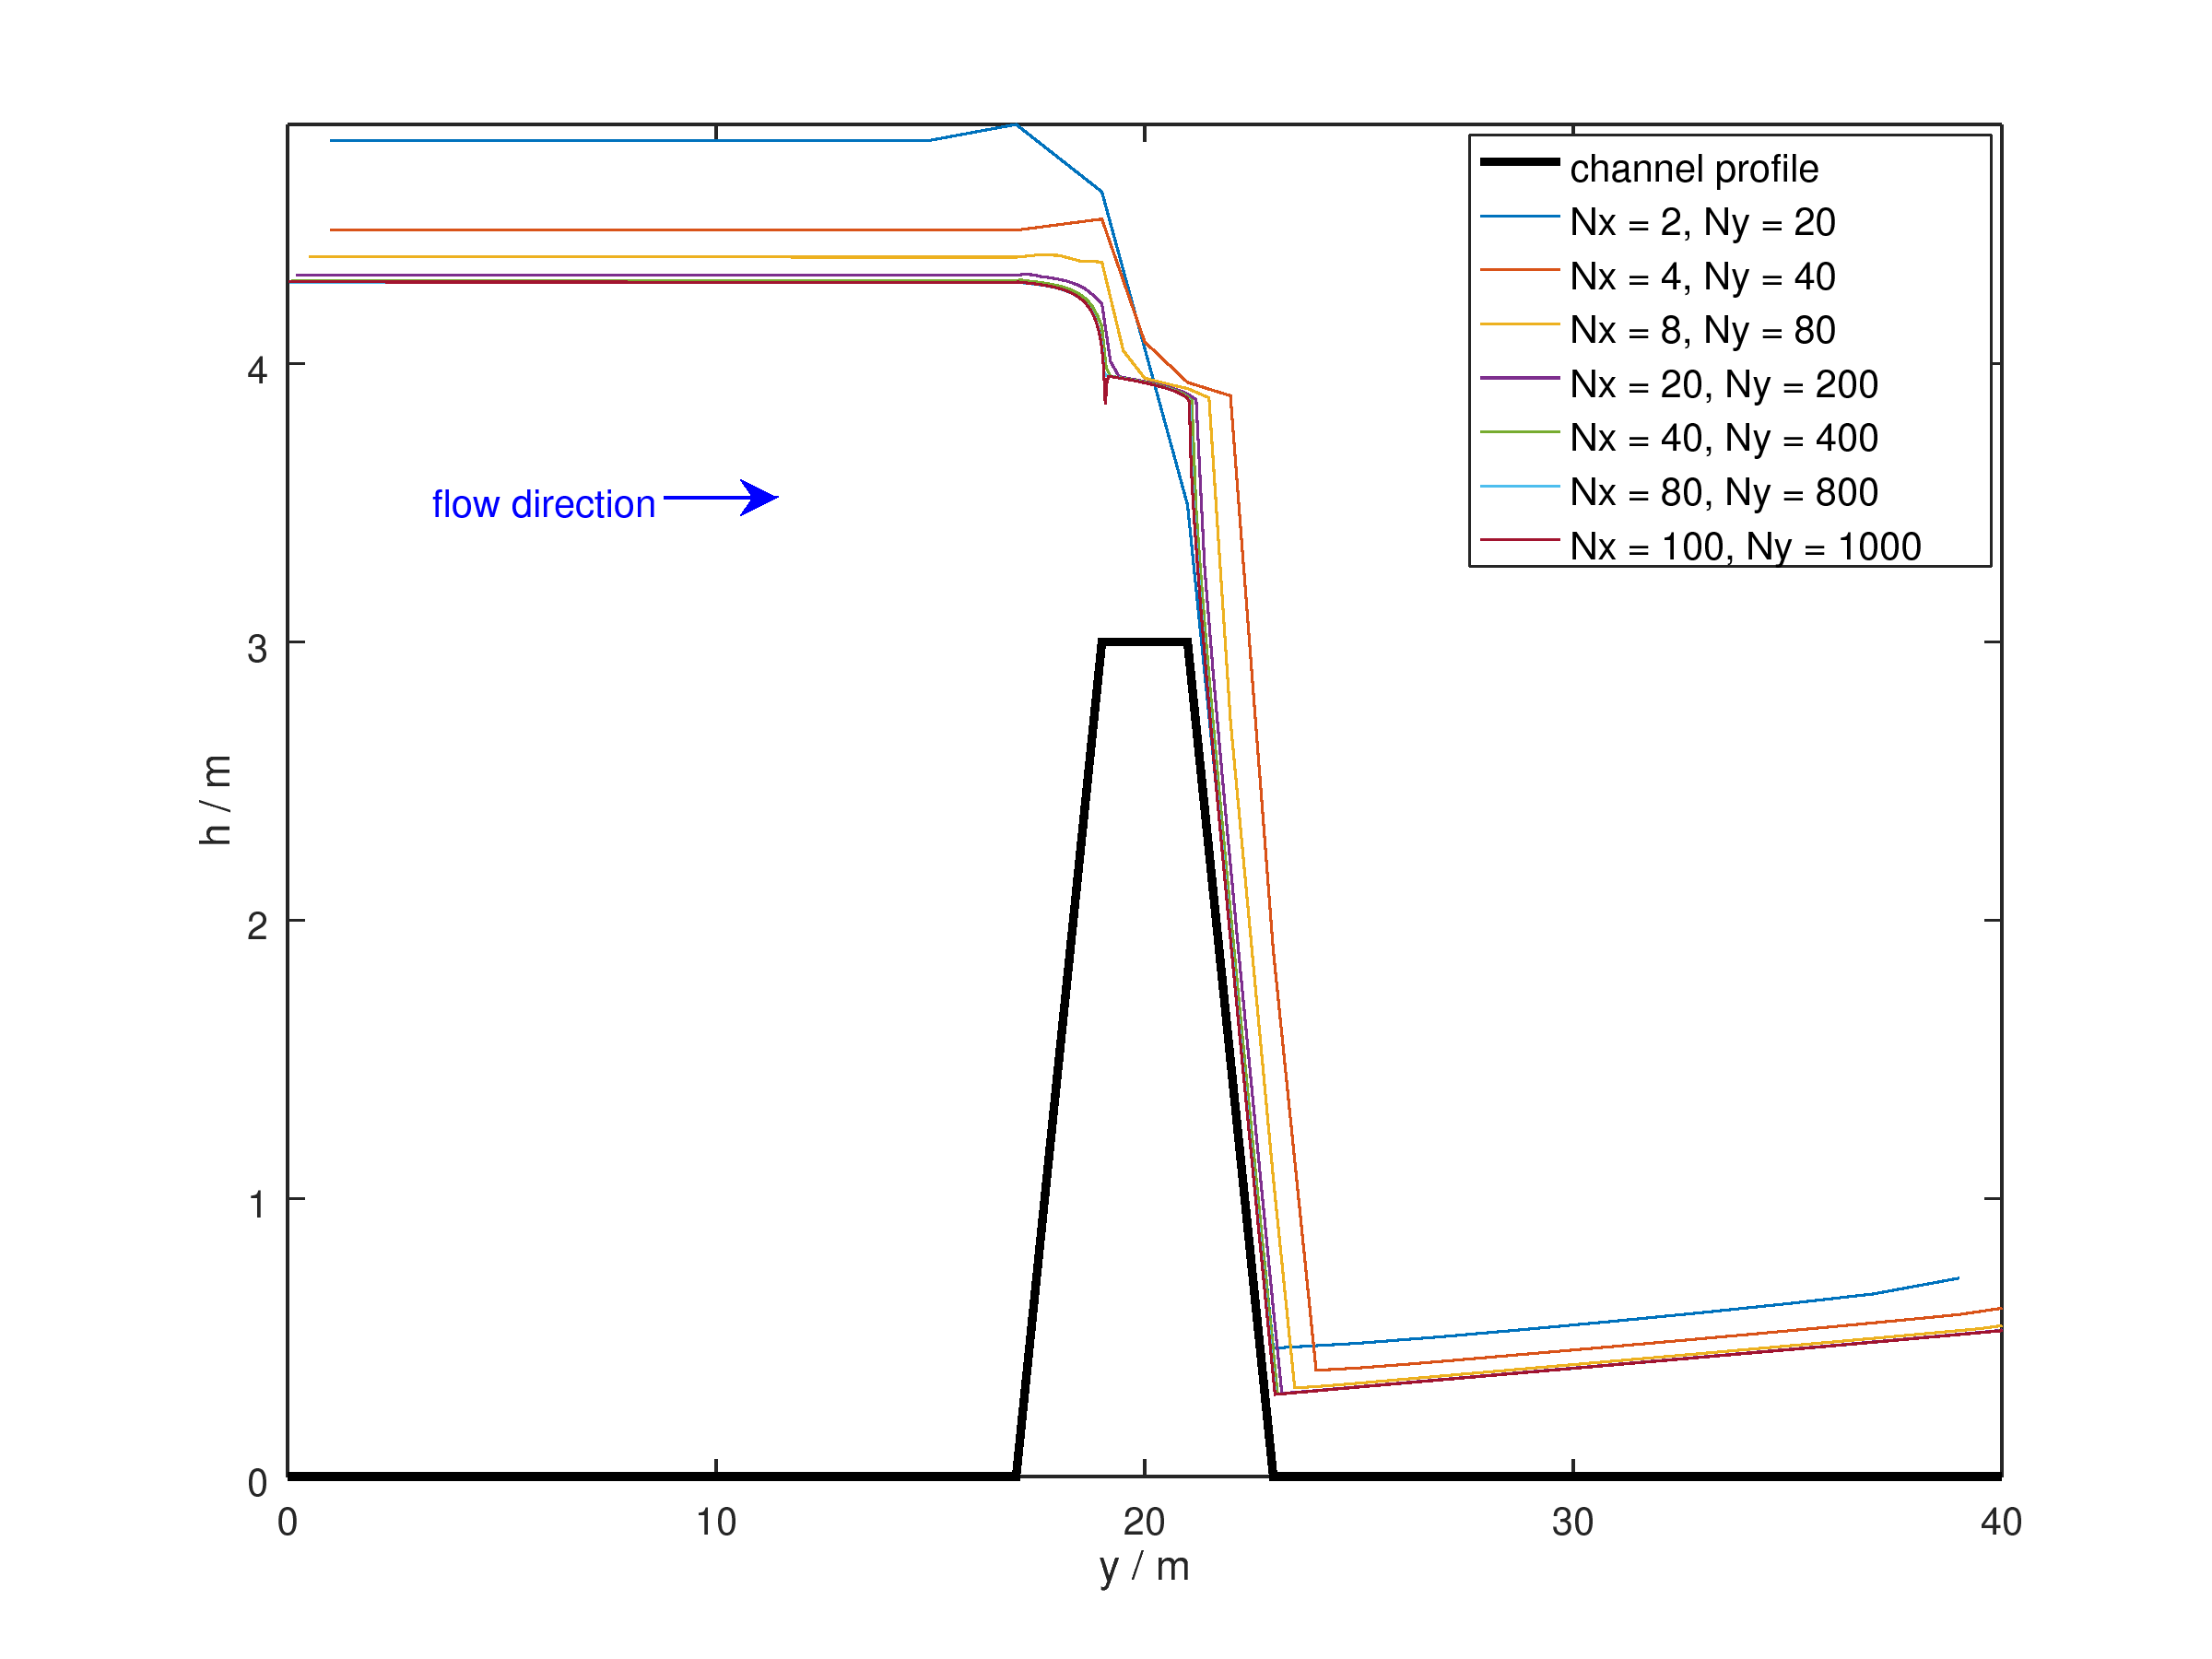
\includegraphics[width=0.7\textwidth]{Figures/water_profiles.png}
  \caption{Longitudinal free surface profiles at steady-state conditions for the \num{7} different grid resolutions. Convergence of the solution for finer grids can be observed.}
  \label{fig:water_profiles}
\end{figure}

In Fig.~\ref{fig:diff_center} the percent variation in the value of $h$ can be observed.
Measured absolute $h$ values at the weir center can be observed in Fig.~\ref{fig:convergence_center} in the Appendix. 
At the \nth{4} refinement the percent variation is smaller than \SI{0.01}{\percent}.
This variation is small enough to assert that the solution has satisfactory converged.
For the experiment it was therefore decided to use $(Nx, Ny) = (\num{40}, \num{400})$ corresponding to a grid resolution of \SI{0.10}{\m} in both x and y directions. The simulation runtime of $\approx \SI{1}{\hour} \SI{10}{\minute}$, required at this resolution is still quite acceptable.

\begin{figure}[h]
  \centering
  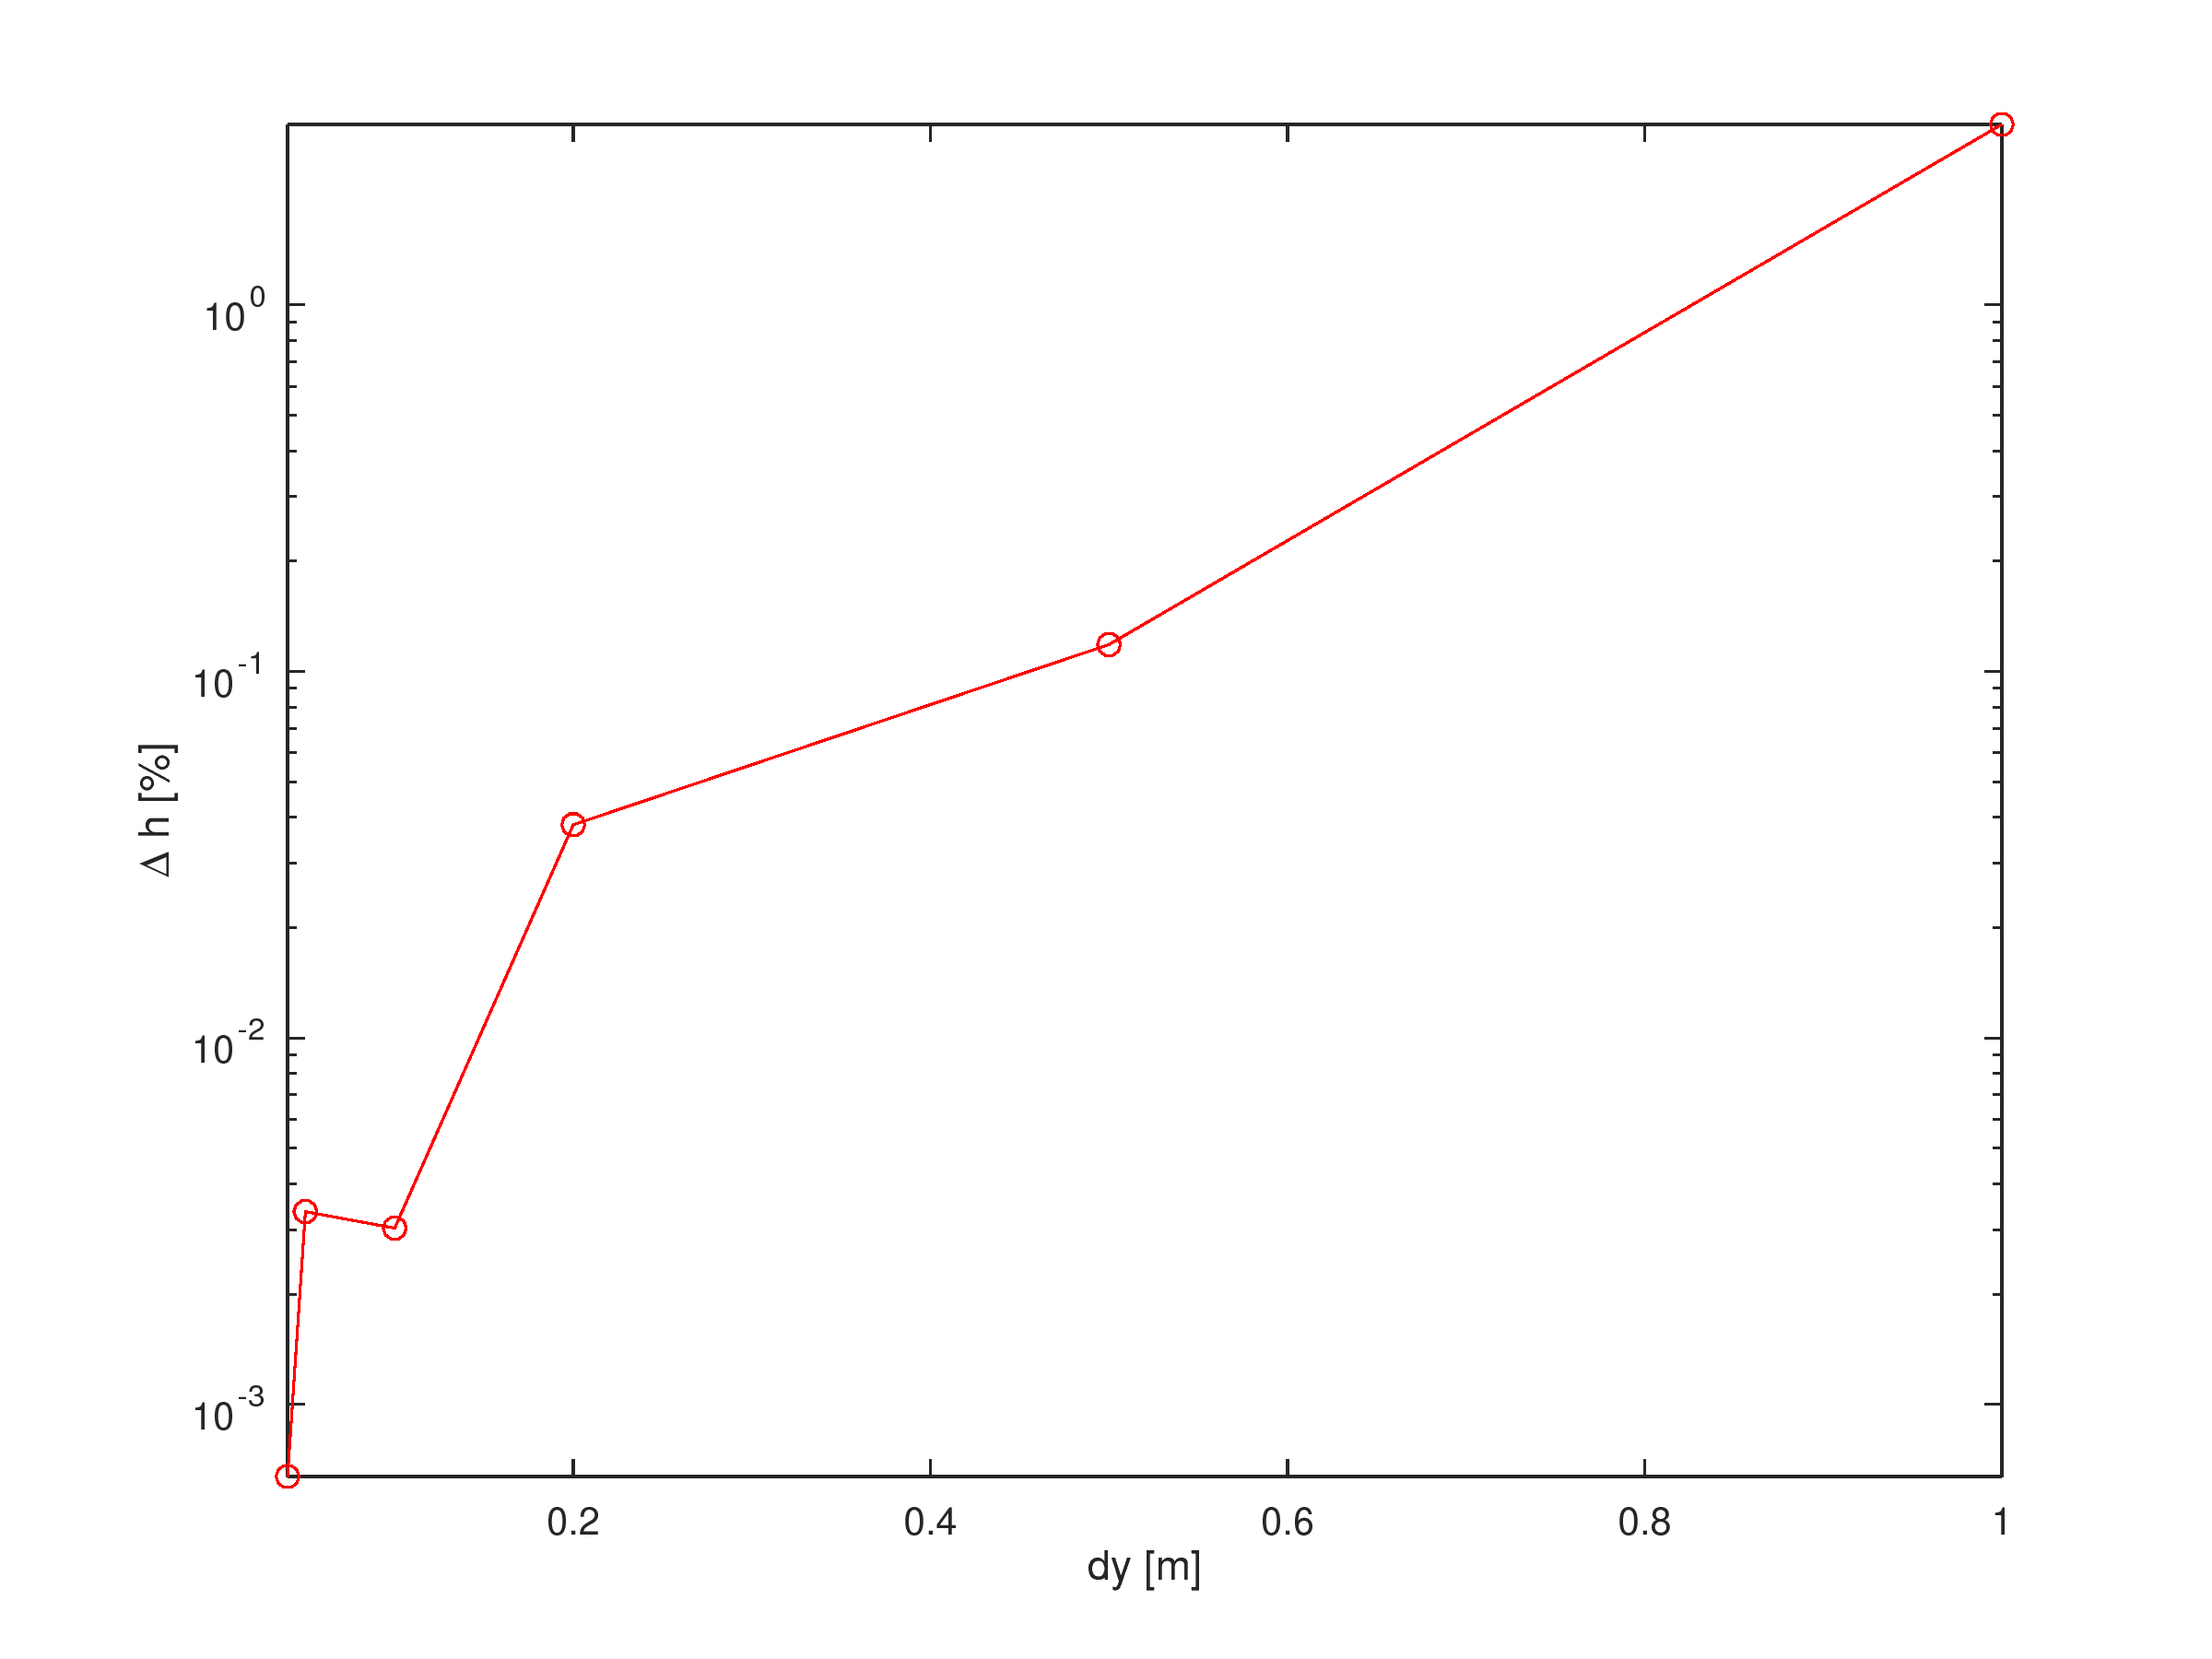
\includegraphics[width=0.7\textwidth]{Figures/diff_center.png}
  \caption{Percent variation of the measured $h$ at the weir midpoint between the given $dy$ and the previous one.}
  \label{fig:diff_center}
\end{figure}


%...............................................................................
\subsubsection{Extracting the dataset}
%...............................................................................
The weir equation computes the discharge over the weir as a function of the water height $h_w$ under steady-state conditions.
These are reached after $\approx \SI{50}{\s}$ of simulation.
After this time, small oscillations of the water surface are still present.
To remove these, a time averaged free surface from $t = \SI{100}{\s}$ to $t = \SI{200}{\s}$ was computed.
Fig.~\ref{fig:free_surfaces} presents the free surface profiles of the \num{25} experiments at steady-state conditions.
The three lowest profiles correspond to the simulation runs with the three lowest inflow discharges. 
As initial condition the weir's upstream side of the channel was filled with water to the weir's height.
The fact that these three profiles are lower than the initial condition is due to a problem with \citetalias{delestre_fullswof:_2017} that lost water from the top boundary.
These simulations were discarded for the continuation of the experiment.
The height value for the remaining simulations was extracted \SI{1.2}{\m} before the weir base, to avoid observations in the acceleration zone, happening in proximity of the weir crest.
At this point a space average over the channel breadth was taken.
The procedure was repeated for all of the experiments.

\begin{figure}[h]
  \centering
  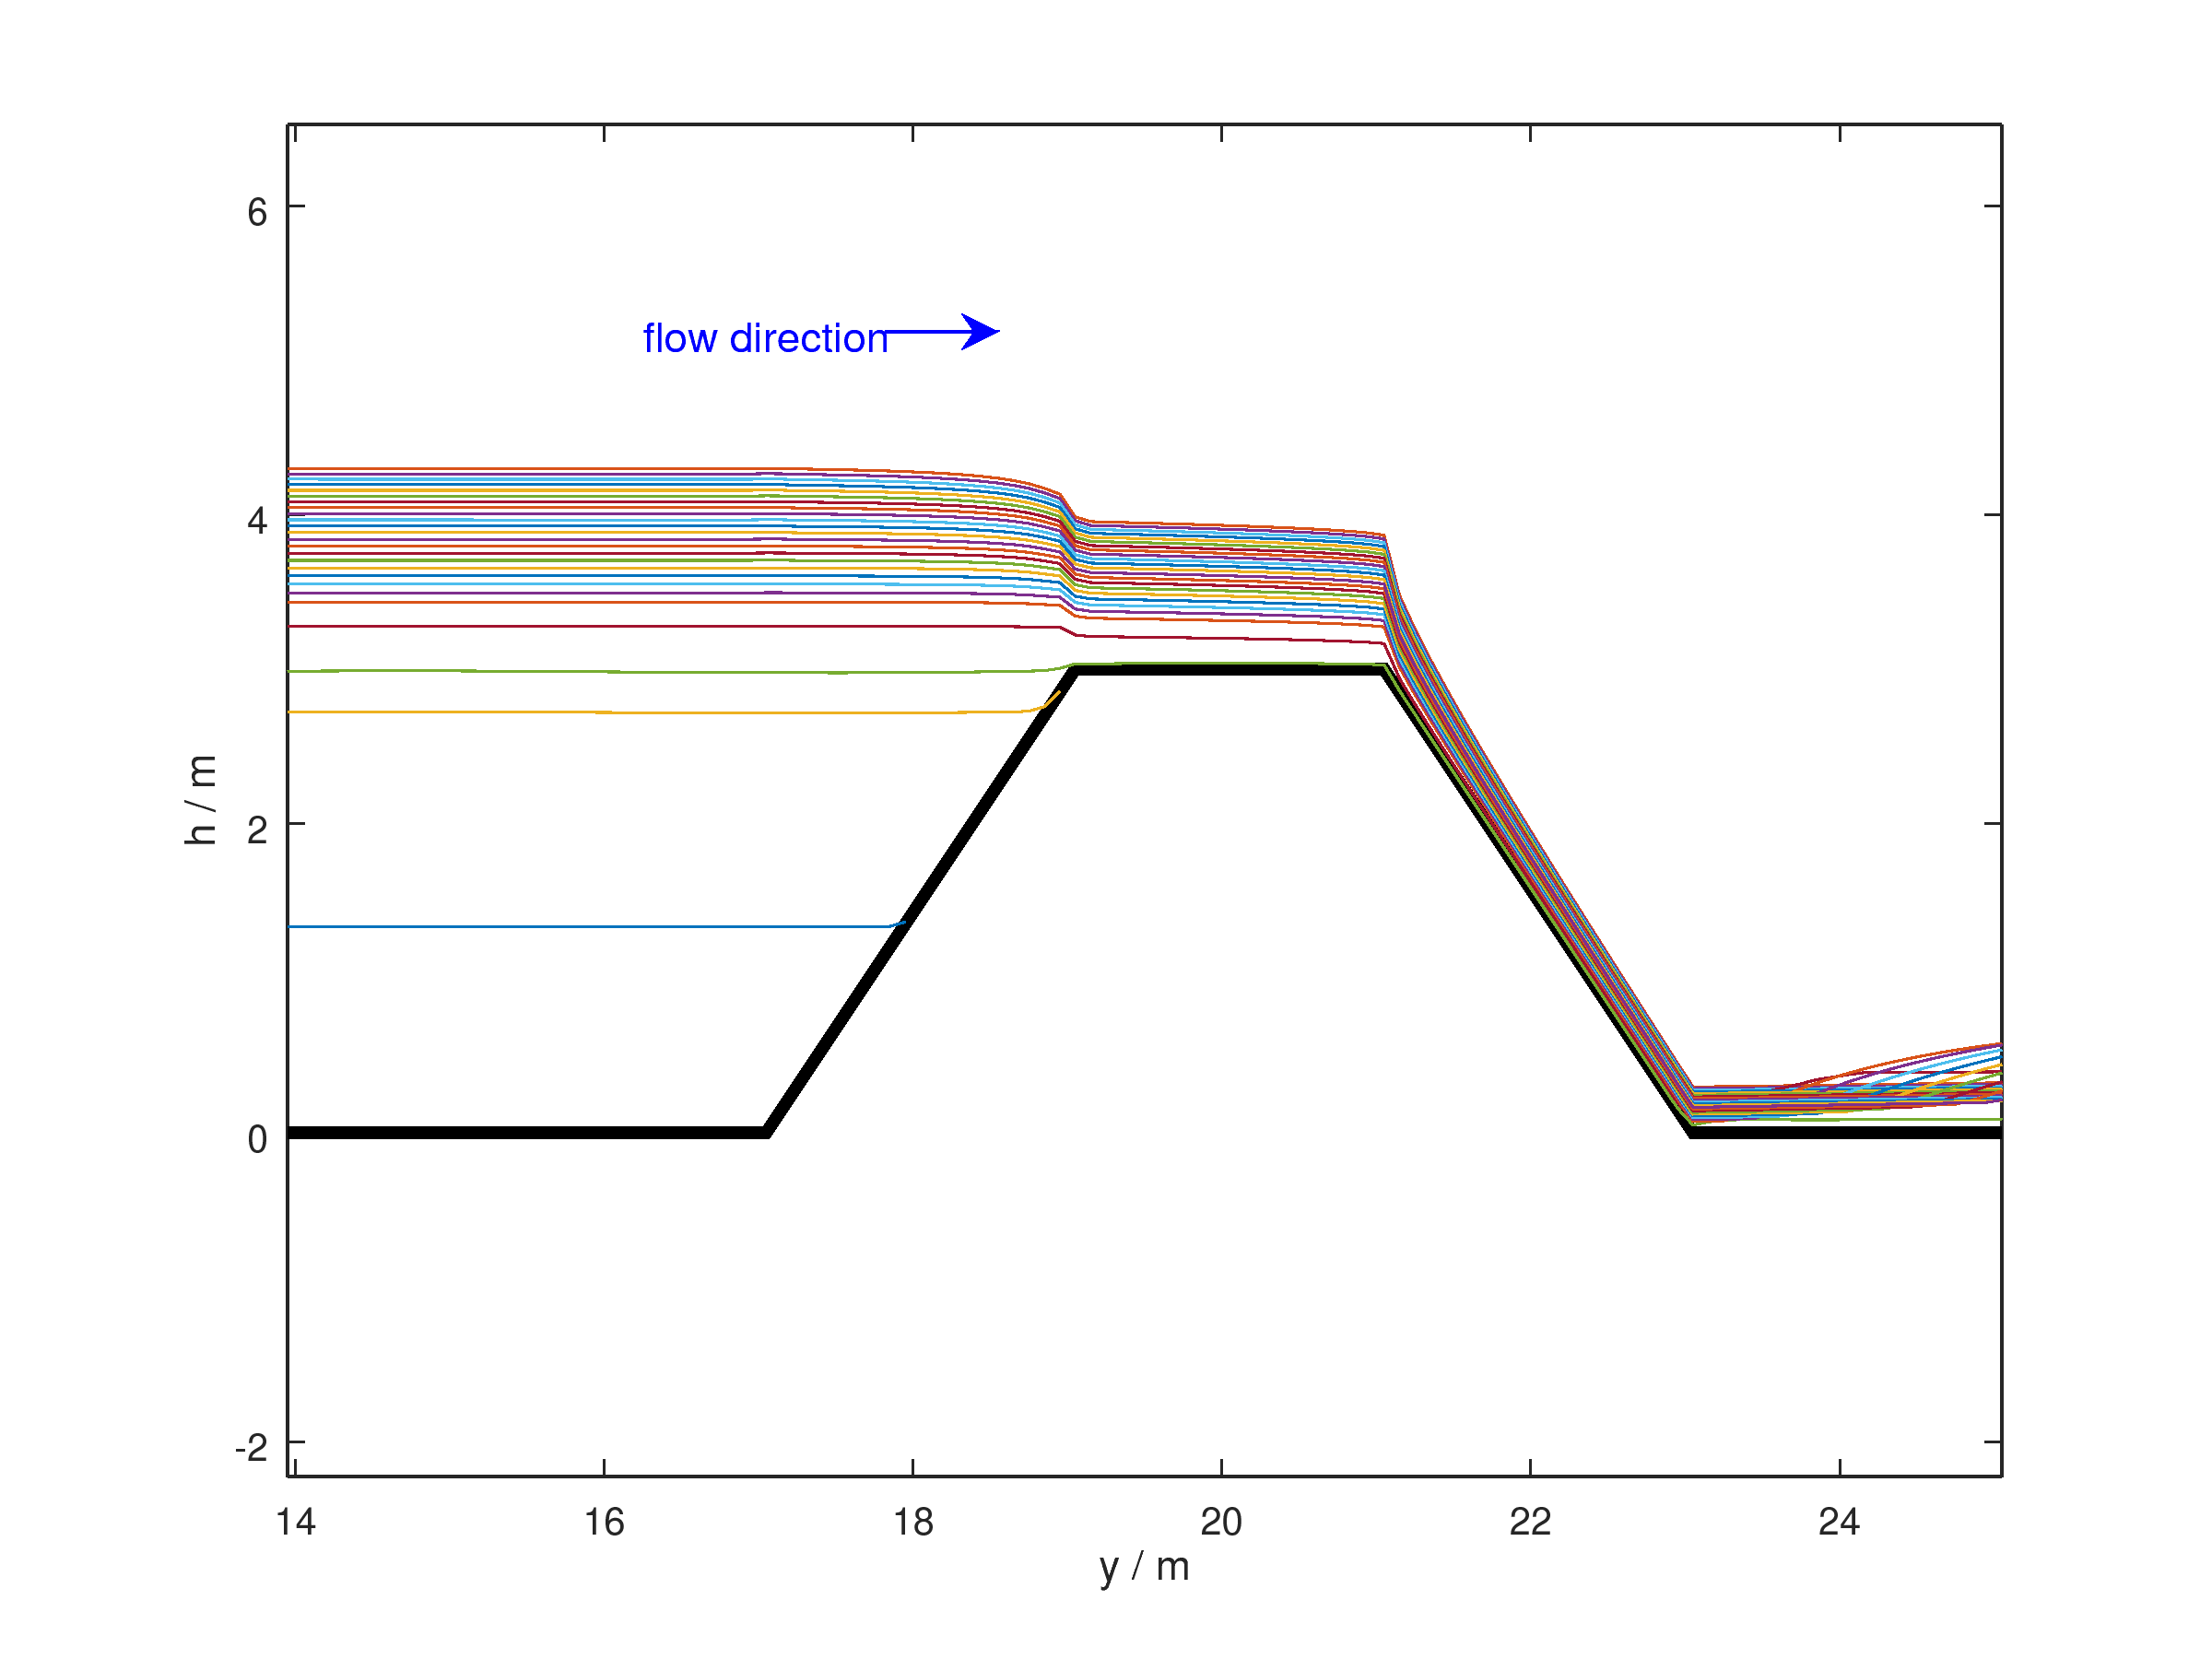
\includegraphics[width=0.7\textwidth]{Figures/free_surfaces.png}
  \caption{Free surface profiles along the channel axis for the \num{25} experiments.}
  \label{fig:free_surfaces}
\end{figure}


%...............................................................................
\subsubsection{Fitting the data}
%...............................................................................
The weir equation (Eq.~\ref{eq:weir_eq}) was fitted to the dataset previously extracted using linear regression.
As the original weir equation is non-linear with respect to the parameters, it was thus linearized by taking the logarithm:

\begin{equation}
  \log(Q) = \log(C) + \log(L) + a \cdot \log(h_w)
\end{equation}

\noindent The values of the parameters $a$ and $C$ were determined from the linearized model.
The performance of the fitted weir equation has been compared with the relationship obtained using linear and cubic spline interpolation.

%...............................................................................
\subsubsection{Computing the error}\label{sec:compute_error}
%...............................................................................
To evaluate the performance of the three models, an increasing number of observations were progressively removed, the models trained on the remaining observations and evaluated on the leaved-out observations.
For an amount $k$ of points removed, all possible combinations were tested. The number of model evaluations follows:

\begin{equation}
  \binom{n}{k} = \frac{n!}{k!\left(n-k\right)!}
\end{equation}

\noindent Since this number grows very fast a subset of the initial dataset was used.
This can be found in Tab.~\ref{tab:dataset_error} in the Appendix.
The first and last points of the dataset were kept during all the \emph{cross-validation} experiment in order to avoid wild extrapolation at the boundaries of the inputs space.
From the remaining \num{12} points all possible combinations of \num{1} to \num{10} points were removed.
The average root mean squared error (RMSE) observed for the removal of \num{1} up to \num{10} points is displayed in Fig.\ref{fig:fitting_errors}.

%-------------------------------------------------------------------------------
\subsection{Results and Discussion}
%-------------------------------------------------------------------------------
% * importance of prior knowledge -> even if few points we can obtain good
%   models. Not the case without (lin. interp, spline interp.)


In Fig.~\ref{fig:simulations_results} the $(Q, h_w)$ pairs extracted from the simulations are plotted.
The gap in the lower part of the plot is due to the data that had to be discarded.
The displayed points represent the input-output sets which was used to fit the weir equation and to apply the  linear and cubic spline interpolation.

\begin{figure}[h]
  \centering
  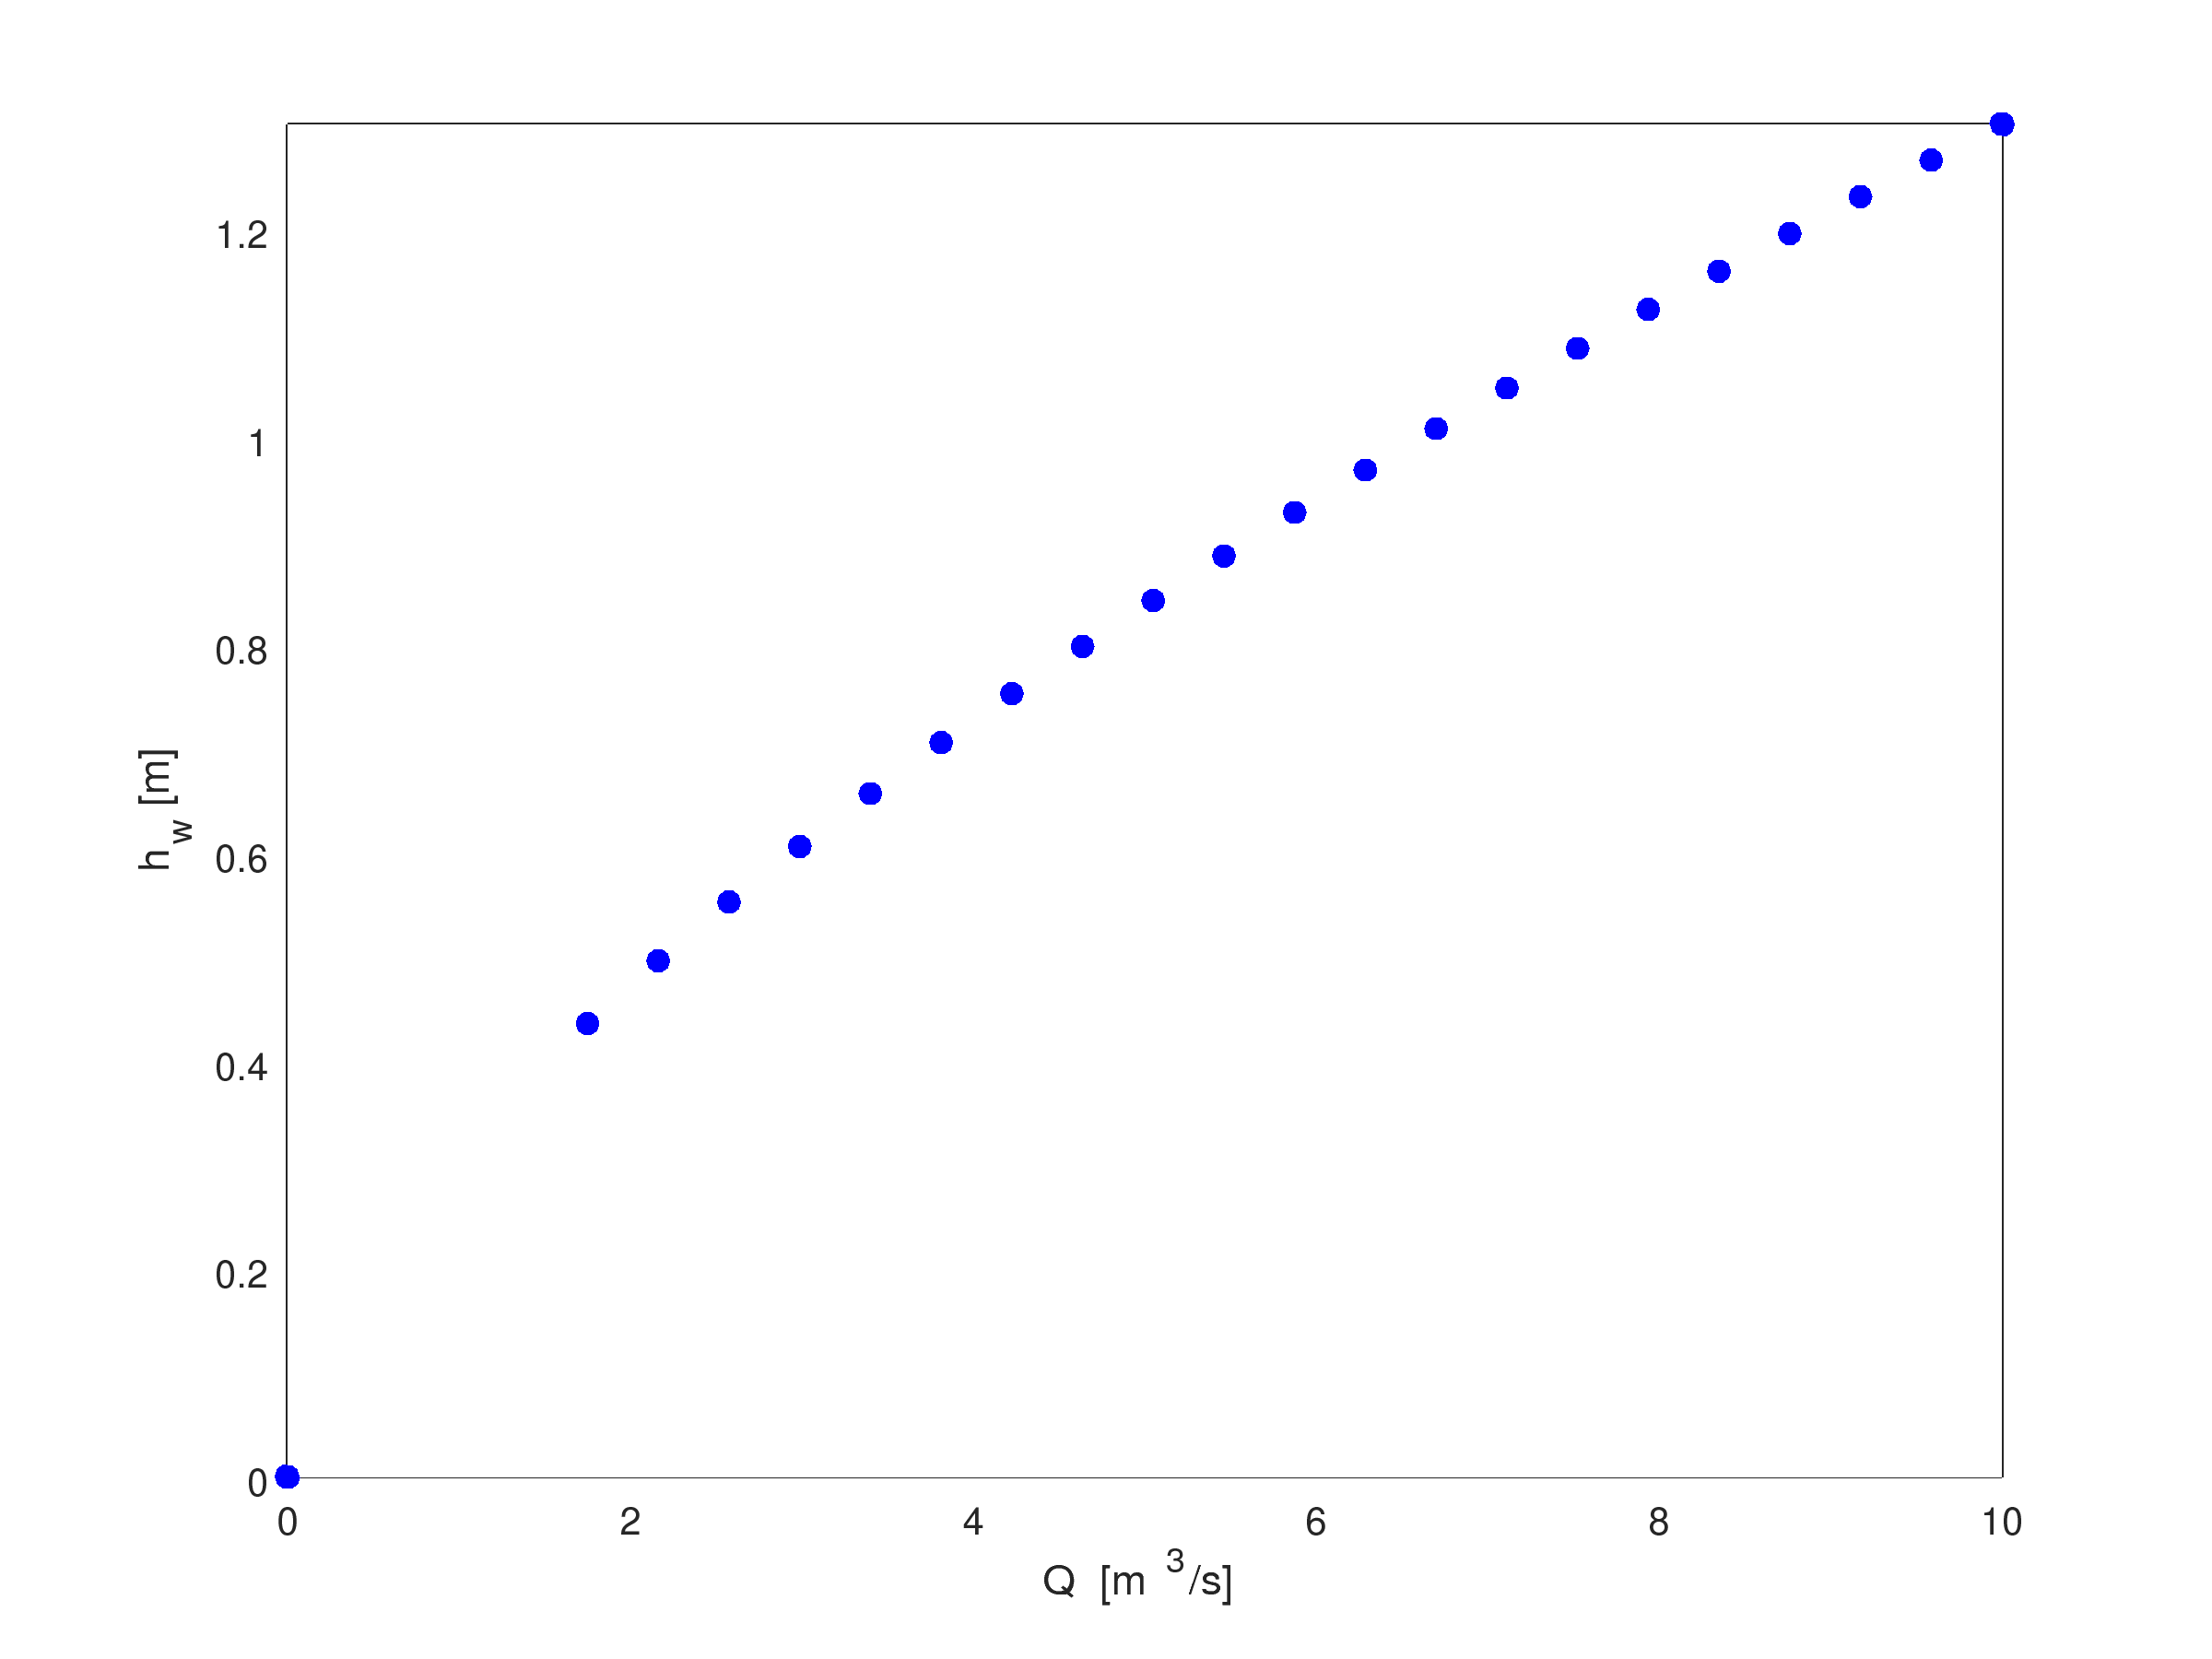
\includegraphics[width=0.7\textwidth]{Figures/simulations_results.png}
  \caption{Plot of the $(Q, h_w)$ pairs extracted from the simulations. Points corresponding to unsuccessful simulations have been discarded, causing the gap visible in the bottom left part of the plot.}
  \label{fig:simulations_results}
\end{figure}

The fit of the different models to the input-output sets is displayed in Fig.~\ref{fig:fitting_results}.
It can be observed that the linear interpolation fails to model the initial curvature which is instead captured by the fitting of the weir equation and the cubic spline interpolation.
This is due to two main reasons. 
First, the density of data points in this region is low---the linear interpolation simply joins the two nearest points with a segment---and on such a long distance it can diverge quite a lot from non-linear models.
Secondly, this region of the input space presents a severe curvature, that makes the linear interpolation to diverge faster.

With the remaining points, all models seem to perform well: the three lines are almost perfectly overlaying, meaning that all give very similar results.
Nevertheless, slight divergences can be observed in proximity of the data points, especially between the weir equation and the two interpolation curves. This is due to the fact that the two interpolation models\emph{interpolate} exactly the points, whereas the curve obtained by fitting the weir equation (which represents the best linear fit to the points minimizing the least-squares-error ), does not necessarily pass exactly through the points.

\begin{figure}[h]
  \centering
  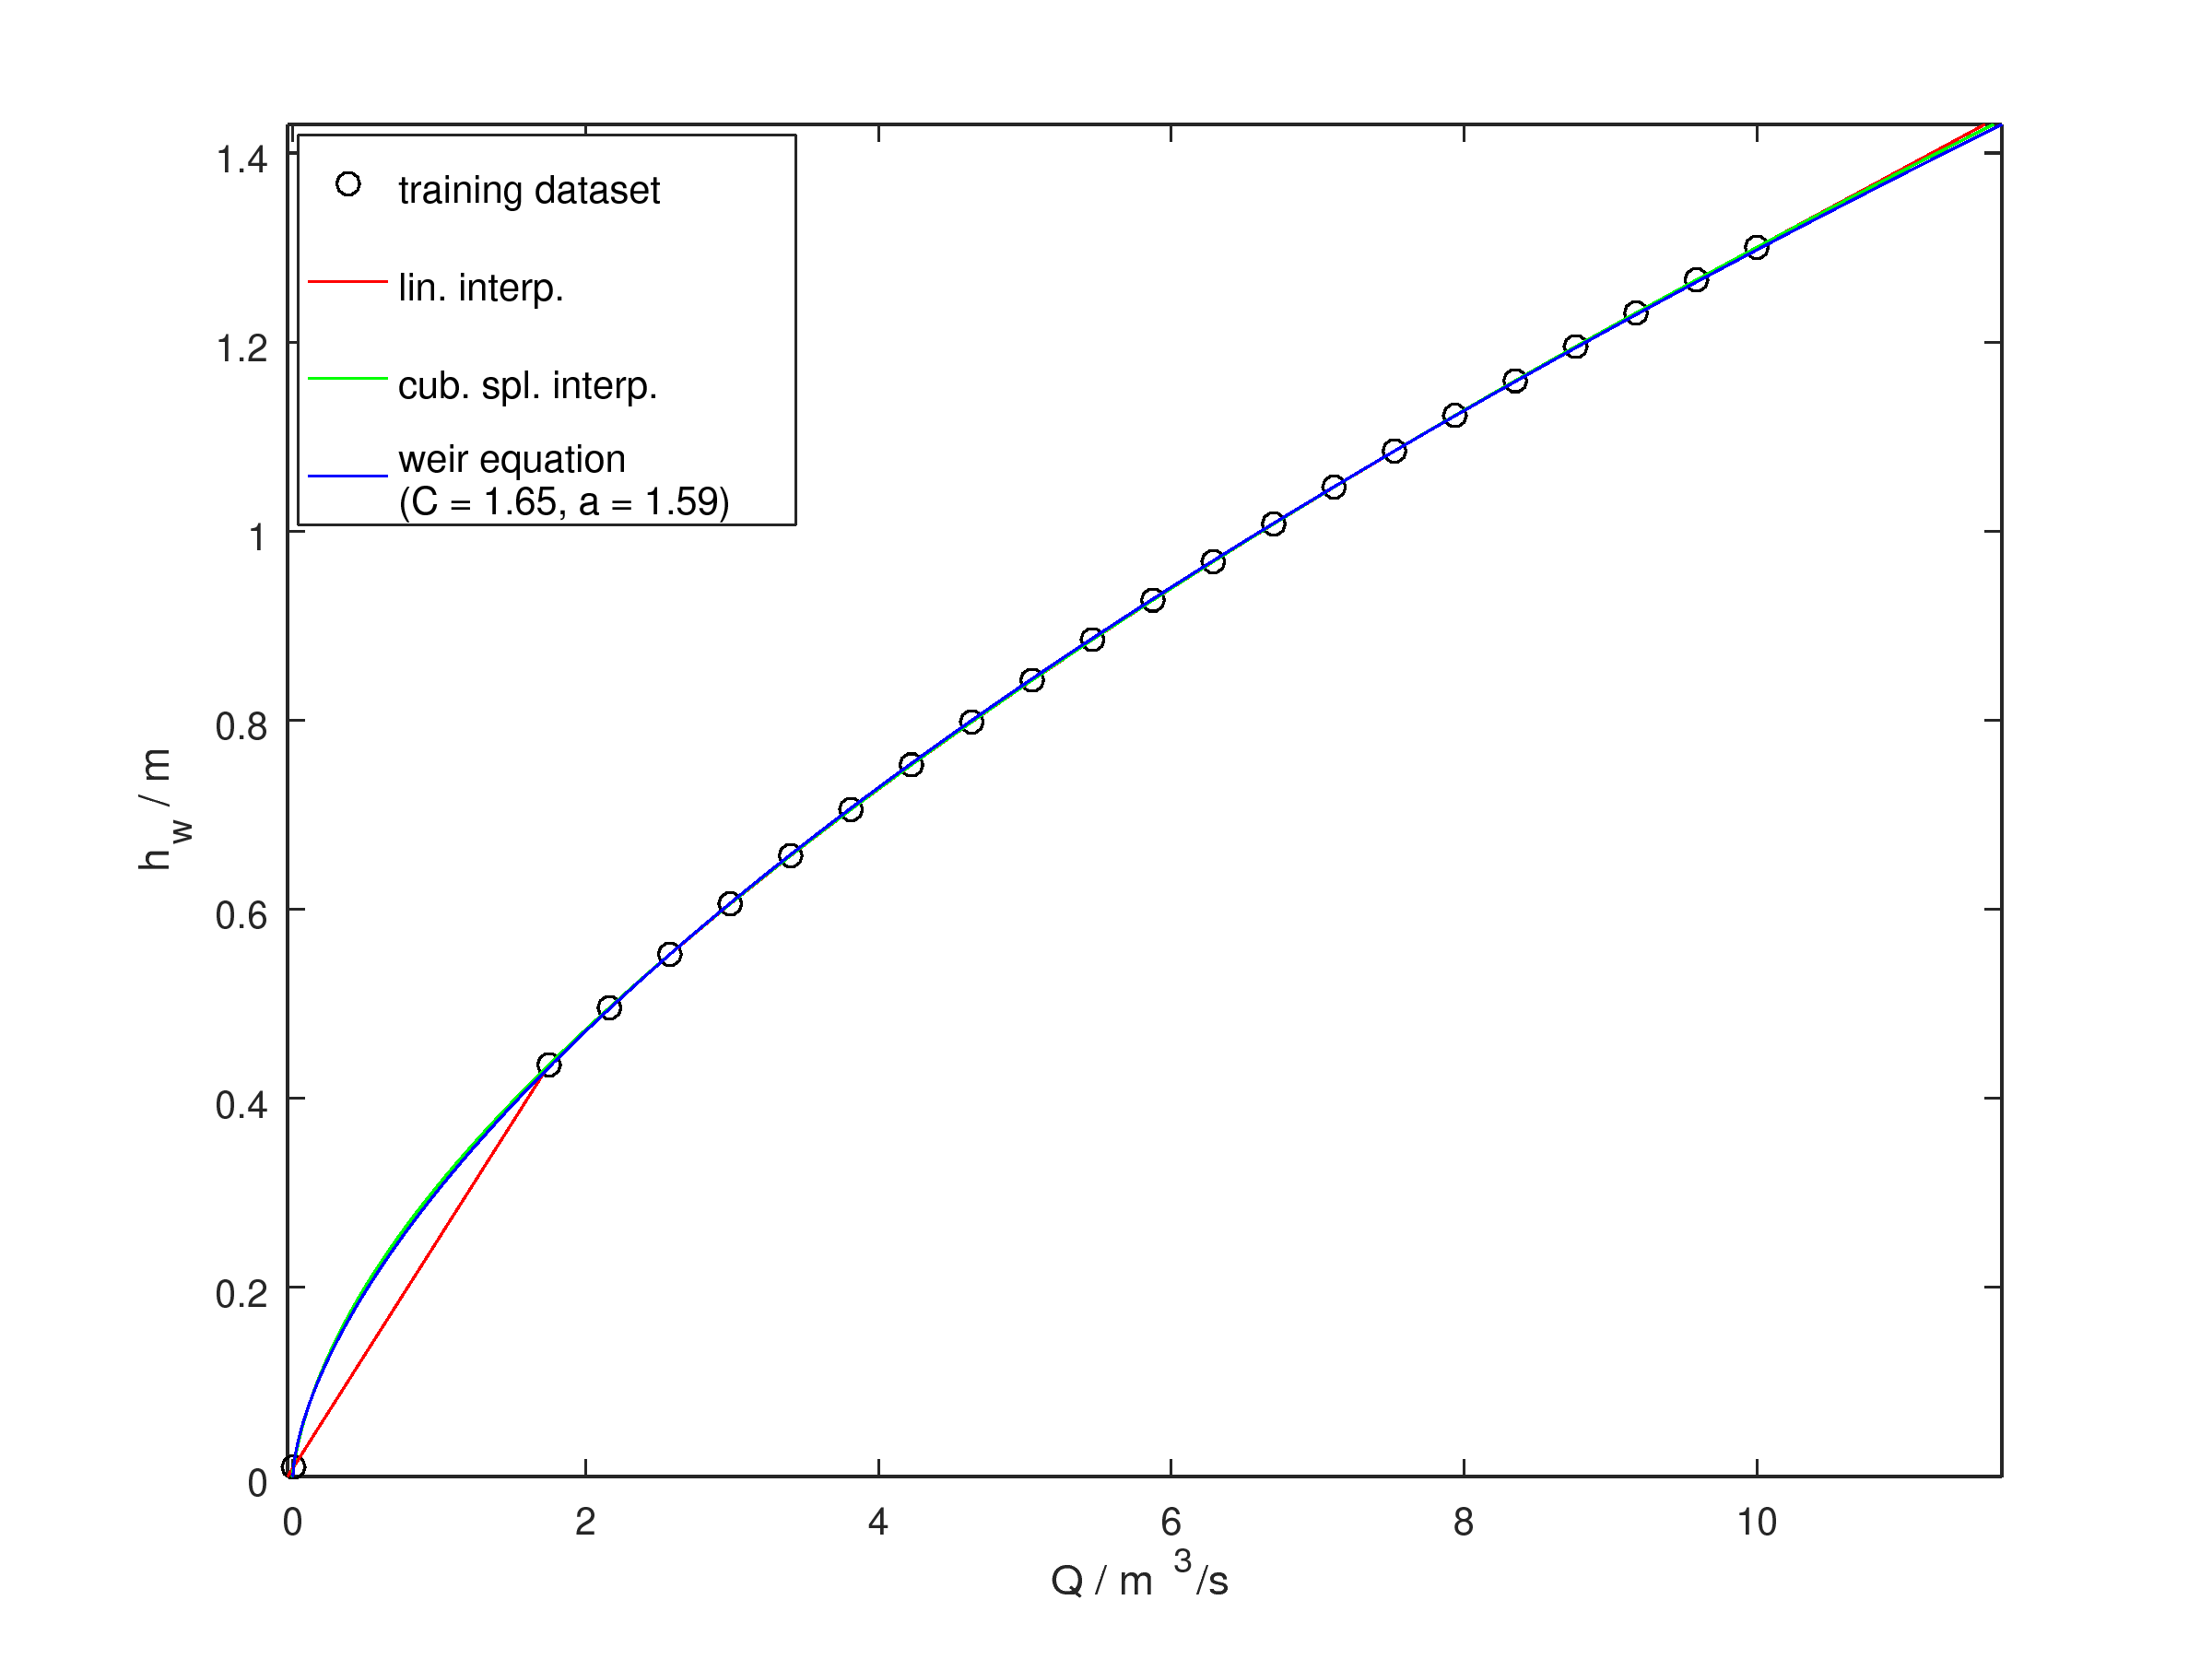
\includegraphics[width=0.7\textwidth]{Figures/fitting_results.png}
  \caption{Fit of the three models to the simulated dataset. In blue the weir equation with $C = \num{1.65}$ and $a = \num{1.59}$, in red the linear interpolation through the points and in green the cubic spline interpolation.}
  \label{fig:fitting_results}
\end{figure}

For the fitting of the weir equation the values $C = 1.65$ and $a = 1.59$ were found.
As mentioned in Sec.~\ref{sec:cs1_brief_description}, for a weir of \SI{2}{\m} breadth and vertical walls, $C$-values in the range $[\numrange{1.36}{1.53}]$ are expected.
The value obtained for $C$ assumes that $C$ does not vary with $h_w$.
Moreover, the weir used for the experiment has a trapezoidal cross section instead of a rectangular one.
\cite{tracy_discharge_1957} investigated how the coefficient $C$ varies with different weir shapes.
For a weir with sloping walls the $C$ coefficient increases, because the head losses in comparison to one with vertical walls are lower.
The difference in the $C$ coefficient observed here can be explained by this phenomenon.\\

\begin{figure}[h]
  \centering
  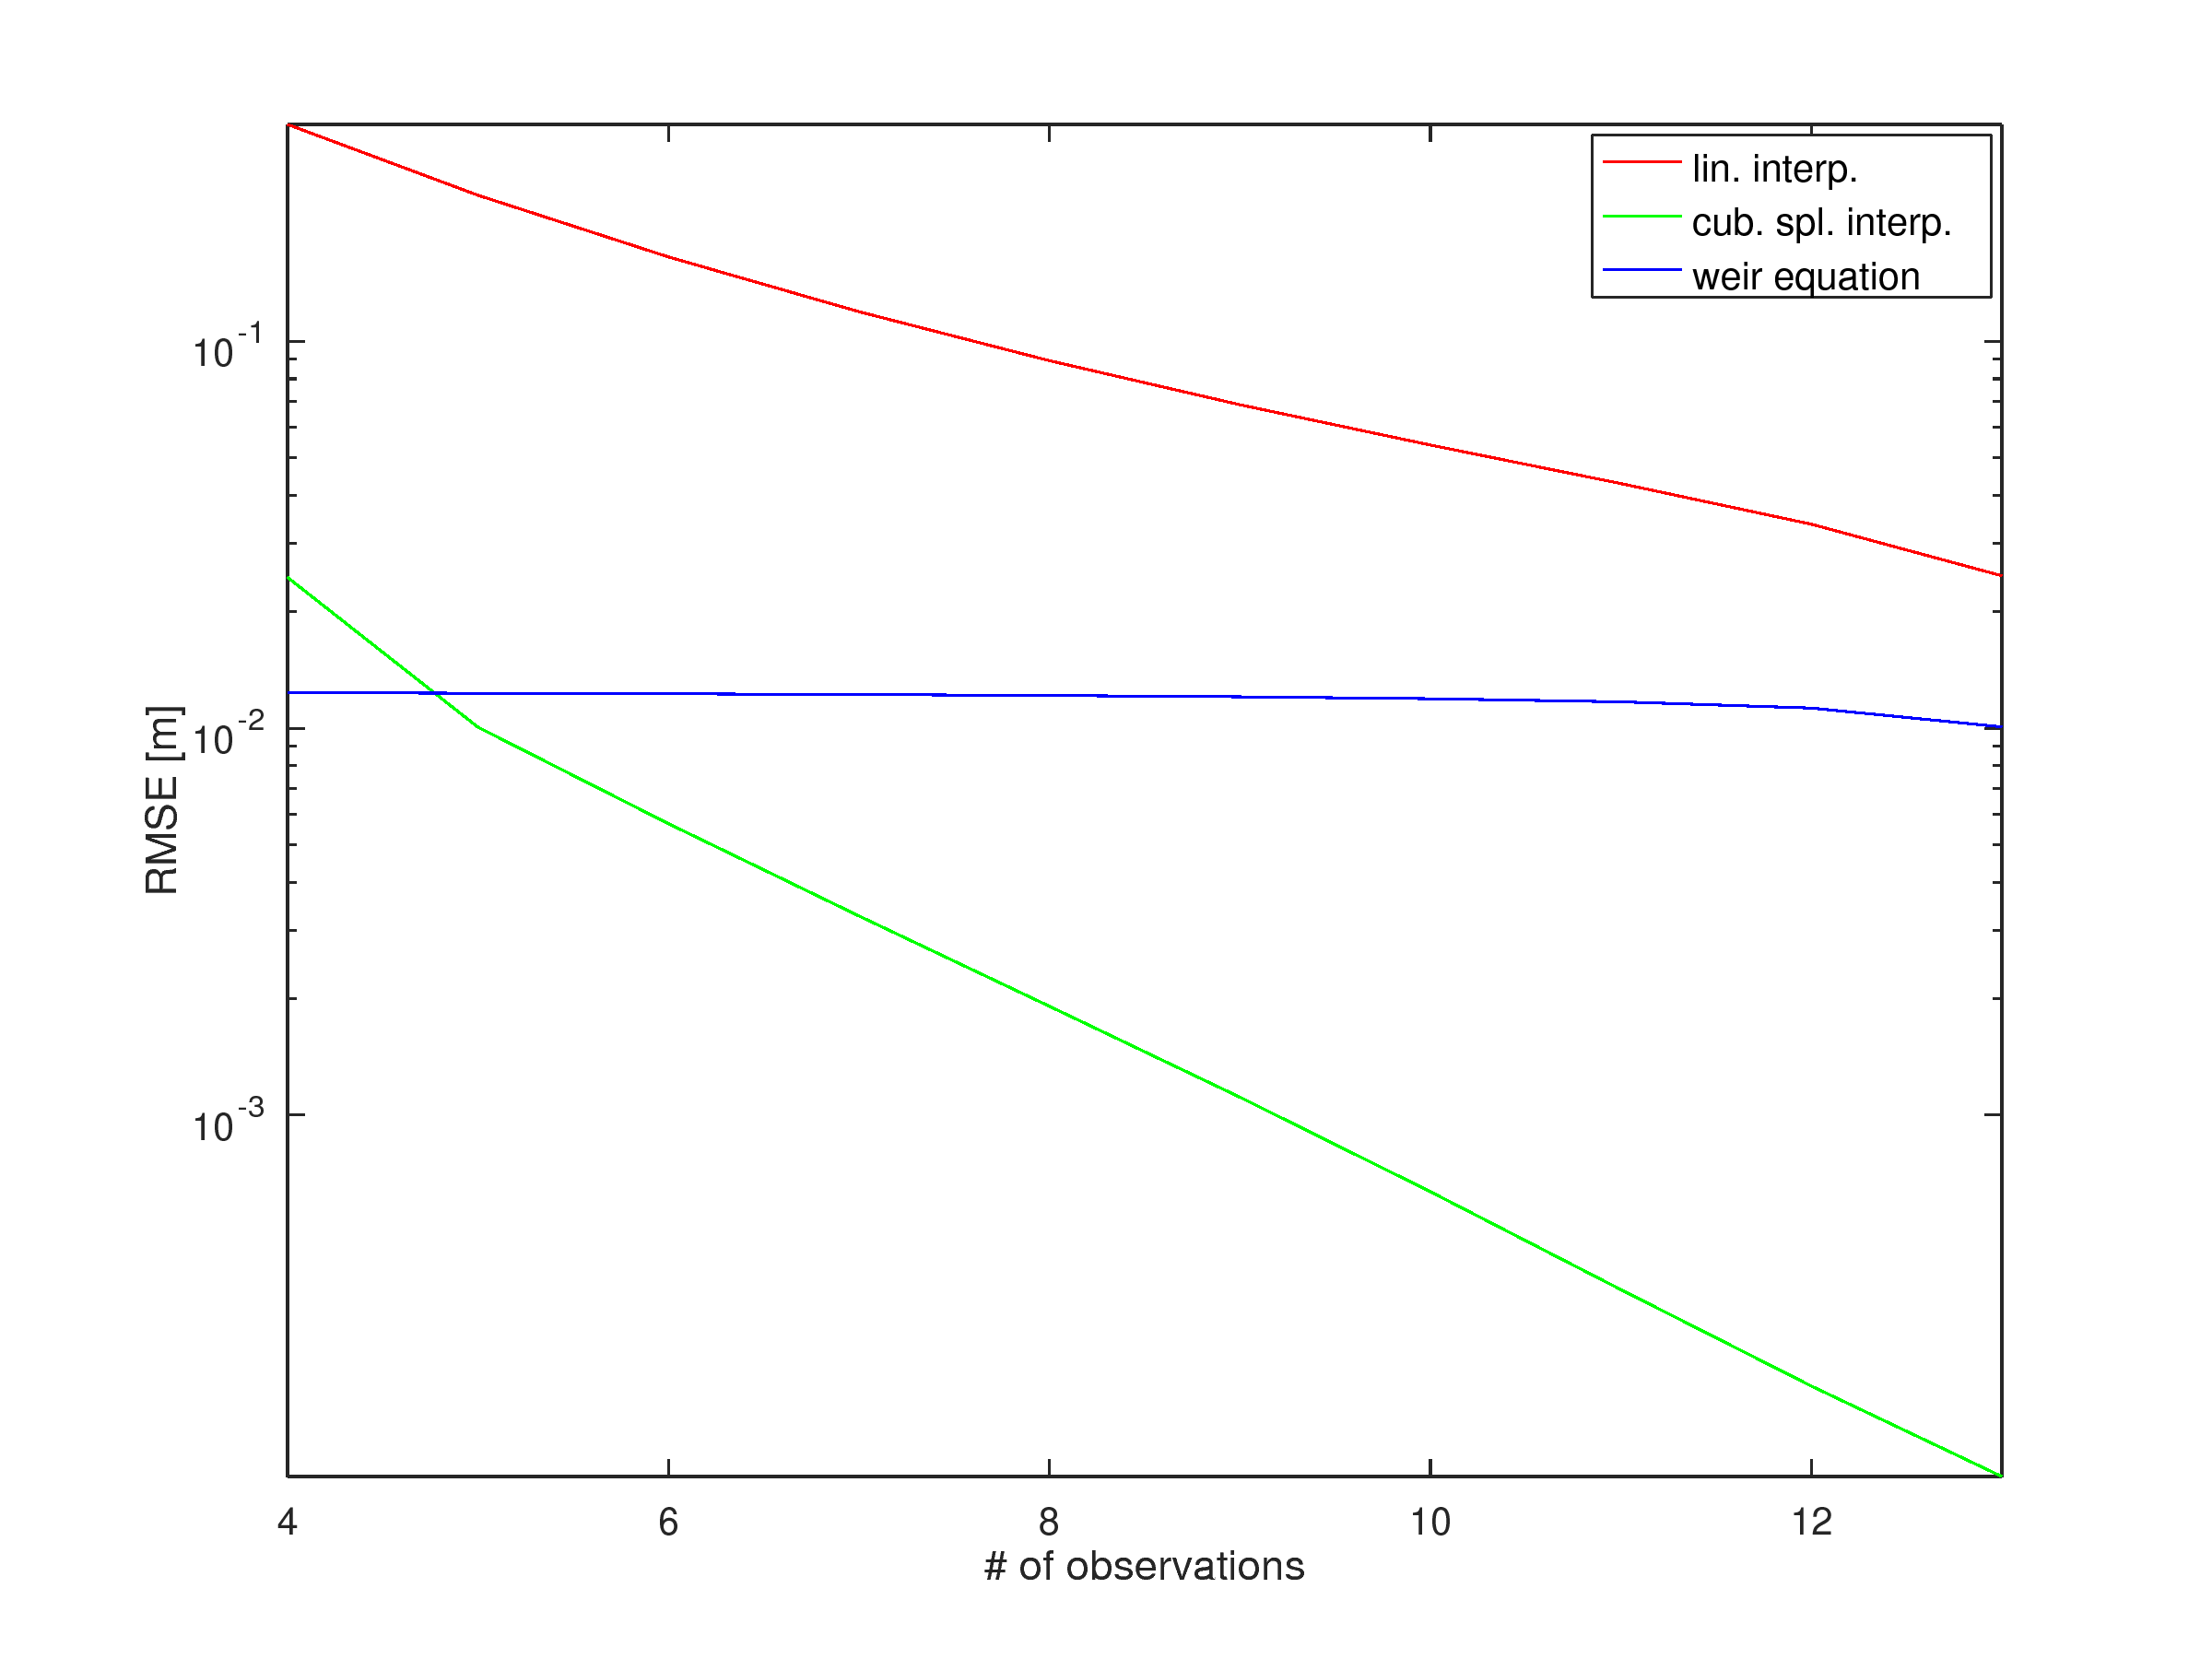
\includegraphics[width=0.7\textwidth]{Figures/fitting_errors.png}
  \caption{Mean RMSE of the three different models as a function of the number of points used to train the models. It can be observed, that the RMSE of the cubic spline decreases exponentially by increasing the number of observations}
  \label{fig:fitting_errors}
\end{figure}

Fig.~\ref{fig:fitting_errors} displays the RMSE obtained by cross-validation as explained in Sec.~\ref{sec:compute_error}.
No matter how many points are used, the linear interpolation always performs worst.
By increasing the number of points its performance improves quite rapidly, but not enough to reach that of the other two models, because the process generating the points does not have a linear behavior.
 
The results for the cubic splines interpolation confirm what was already observed in Fig.\ref{fig:fitting_results}:  cubic splines interpolation seems to mimicks in an accurate manner the process originating the points.  This is explainable by the high flexibility of cubic splines interpolation method, which typically shows very small errors when fitted with many points. However, by reducing the number of points available for interpolation, the error of this model increases exponentially. Despite this, on average if more than 5 observations are available, cubic splines interpolation outperforms the other methods.

On the other hand, the regression line obtained using the weir equation model shows only a slight decrease in accuracy when progressively removing observations for fitting. This high stability (insensitivity to the number of available observations for fitting) is due to the fact that in this case only two regression coefficients must be determined. Nevertheless, the low flexibility of linear regression models tends to prevent the interpolation of the data points and causes the linear regression model to not outperform cubic spline interpolation when many observations are available and the functional relationship is non-linear (or not optimally parametrized by an ad-hoc equation).  

%The weir equation model used minimizes the least-square-error of the fit, without necessarily interpolating through the points.
%It is a very inflexible model, as only two parameters can be varied to improve the quality of fit, while many more observations are available.
%For this reason, the interpolation through the points cannot be achieved, unless the observations were originated exactly by the model chosen.
%Because interpolation cannot be obtained, its error decreases very slowly with increasing number of points.
%The inflexibility of this model represents its weakness but at the same time its strength.
%This is in fact a very robust model, which still produces good results when few observations are available.
%It shows almost no decline in performance by reducing the number of points.

Fig.~\ref{fig:boxplot_models} in the Appendix summarizes the performance of the three models when using $[\numrange{4}{13}]$ \# of points.
Here it can be seen that the RMSE for the weir equation is higher on average respect to the cubic spline interpolation but still quite low (in the order of $\approx \SI{1}{\centi\meter}$).
Its variation is almost inexistent; the box plot is practically described by a line.\\

An in-depth comparison between the two best models (see Fig.~\ref{fig:fitting_std}) shows new interesting features.
The cubic spline interpolation is very sensitive to which points are removed when few observations are available for interpolation. The standard deviation on its RMSE by changing which observations are removed increases by a factor of \num{60} when \num{4} resp. \num{13} points are used.
Oppositely, the regression line based on the weir equation model is more sensitive to which observation is removed when only few of them are removed; while it becomes less sensitive as fewer observations are used to fit the model. However, the variation in RMSE variability  when \num{4} resp. \num{13} points are used, change only by a factor of $\approx \num{6}$.

When considering this, the regression line based on the weir equation can still have the potential to perform better than the cubic spline interpolation when only up to \num{6} observations are available (and not just by \num{4} as it was indicated by Fig.~\ref{fig:fitting_errors})

In the weir equation model proposed by \cite{brown_urban_2009}, the coefficient $C$ has been allowed to varies as a function of $h_w$:  the shorter the weir width, the wider becomes the range of values for the $C$ coefficient. If the regression line would have been fitted on this model, then a better fit to the observations would have been obtained.

\begin{figure}[h]
  \centering
  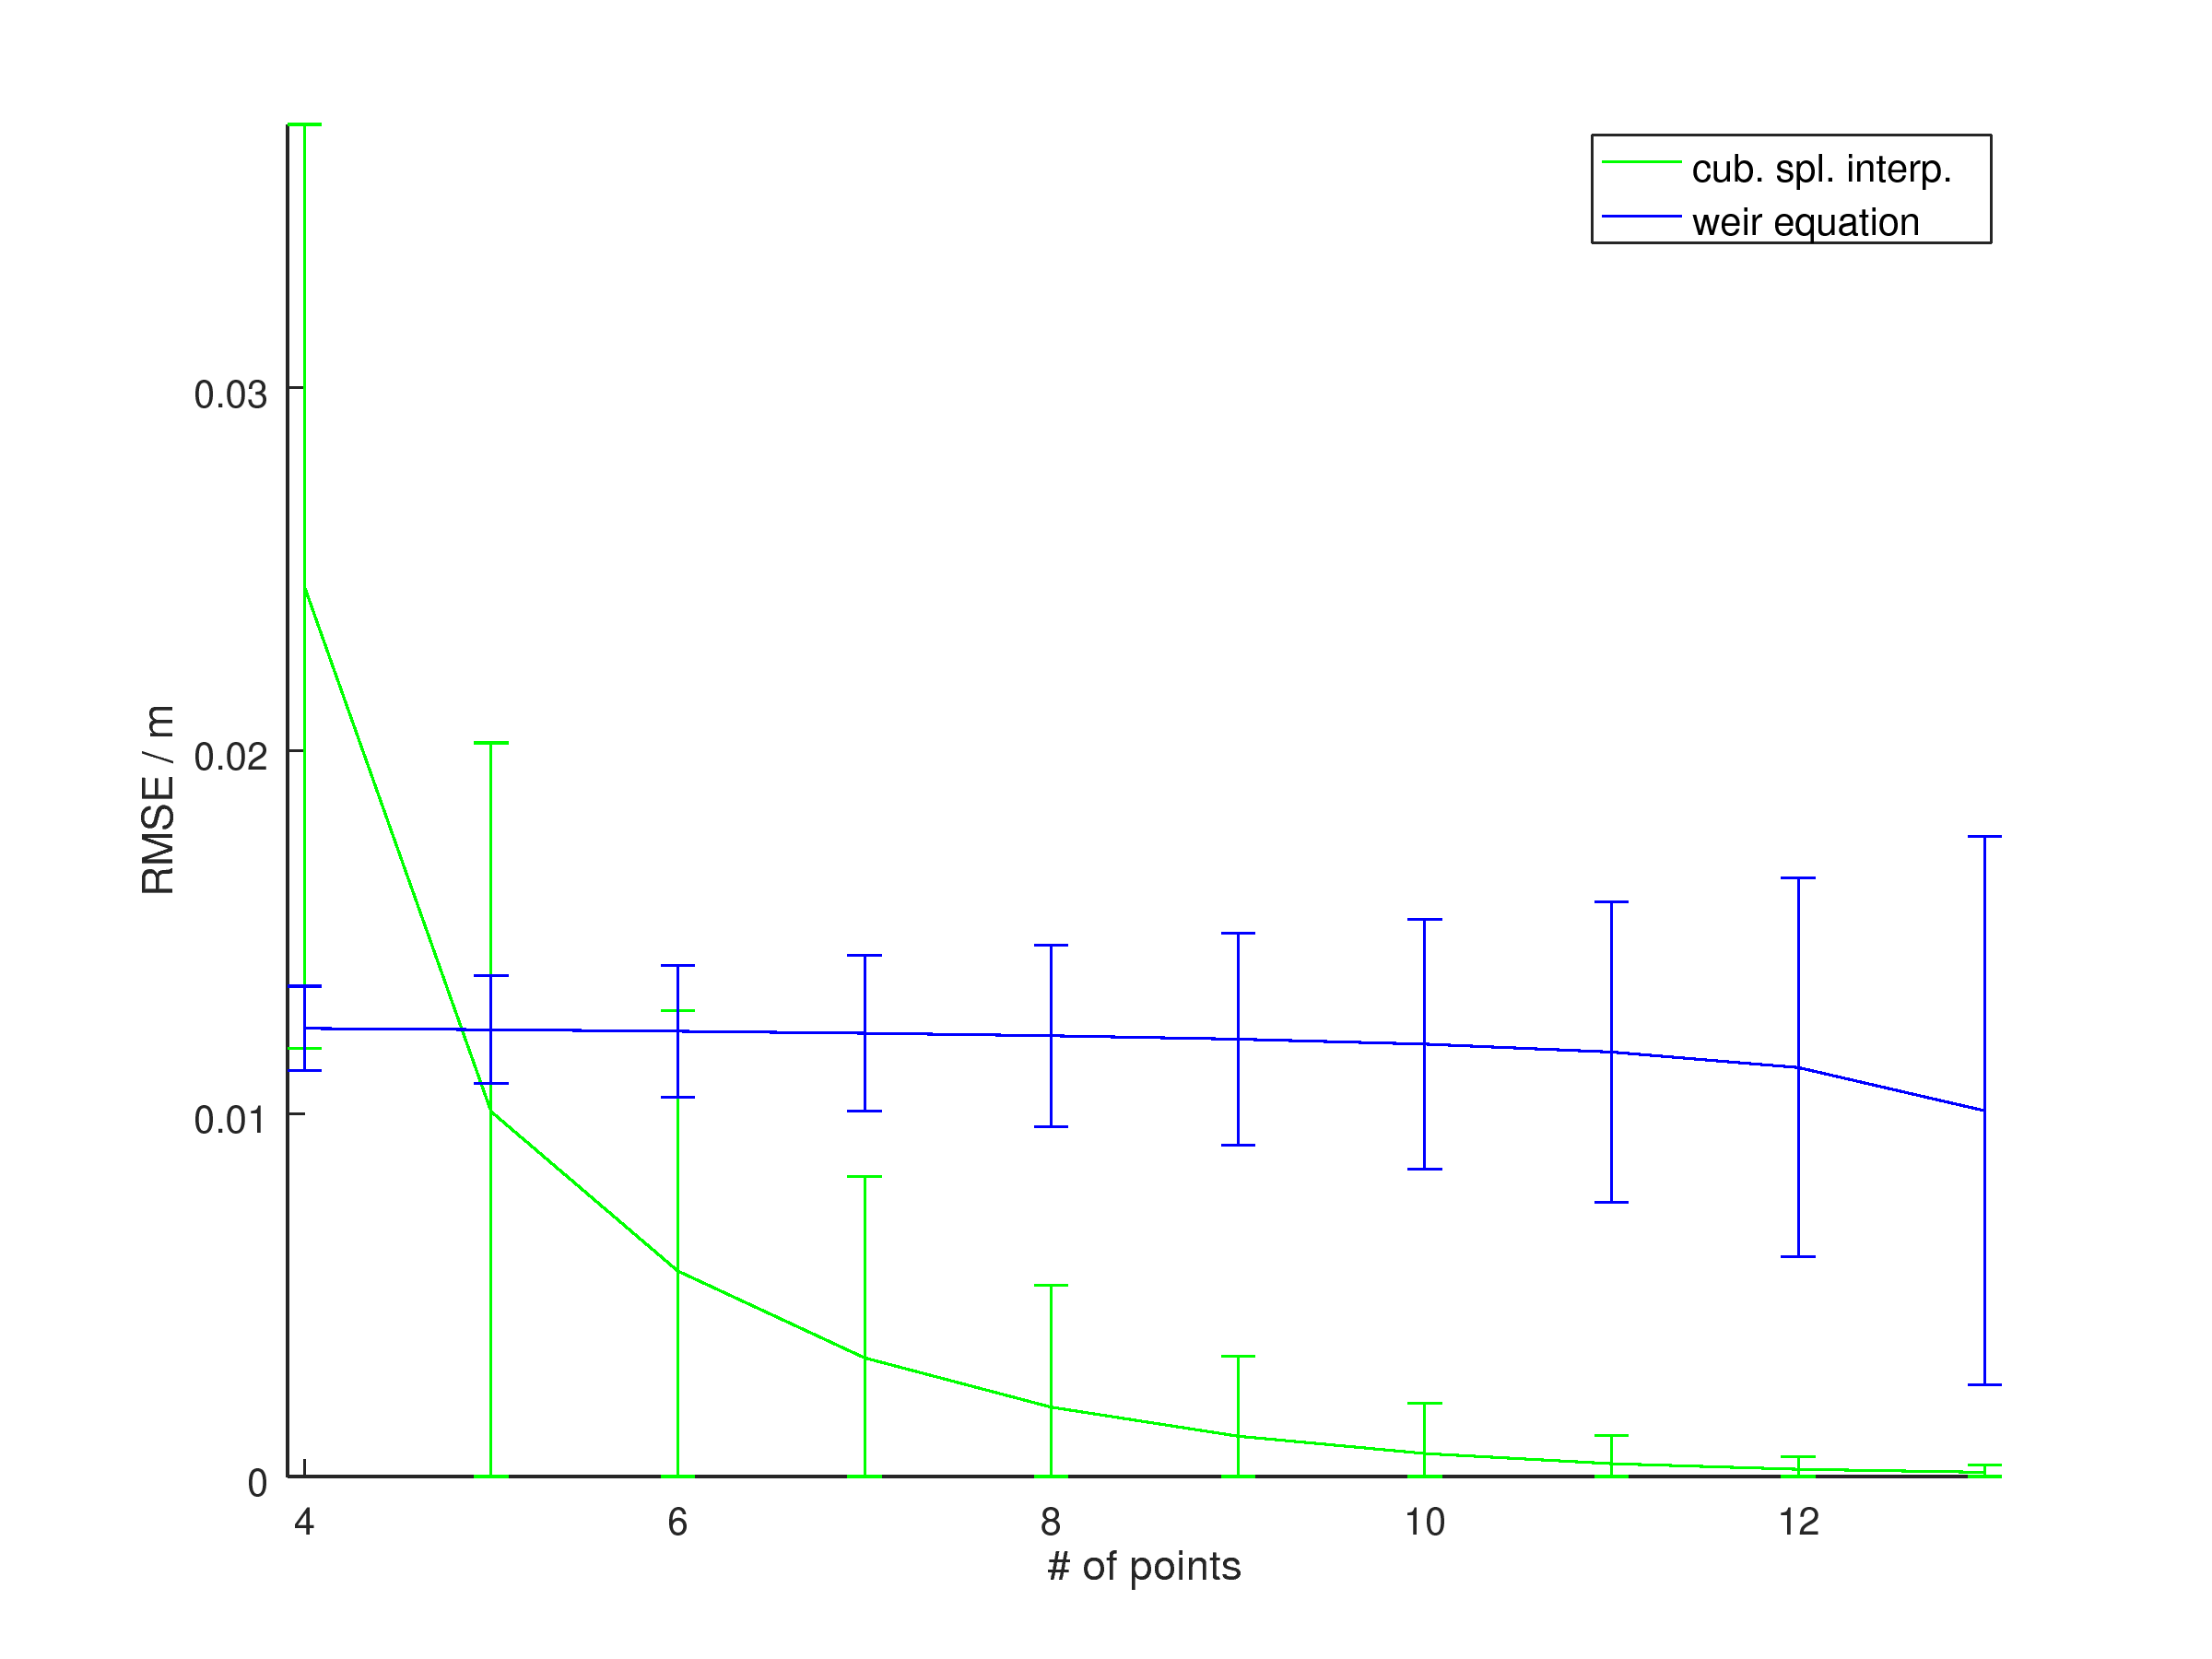
\includegraphics[width=0.7\textwidth]{Figures/fitting_std.png}
  \caption{Closer comparison of the weir equation and the cubic spline interpolation models.}
  \label{fig:fitting_std}
\end{figure}


This first case studies highlighted the importance of the trade-off between \emph{prior knowledge} and \emph{data availability}.

Machine learning (ML) regression algorithms such as \emph{RandomForest} (Breiman et al.), \emph{Gradient Boosting Machines}(CITT) and \emph{Feedforward Neural Networks}(CITTT) are known to be very powerful on establishing non-linear functional relationship hidden in the data, but they also are particularly data-greedy. They have the potential to perform very well when a big training dataset is available, but fail if not enough data are available. Using numerical simulators, the generation of these large training datasets can be computationally very costly, thus partially hampering the use of these algorithms.

In this case study, we showed that simpler interpolation methods can still allow to obtain good performance when  moderate simulated input-output sets are available. 
Moreover, the encoding of prior knowledge was proved to be useful when less data are available: the \emph{weir equation} model, unlike the others, could still perform well when fitted to few observations.

Taking into consideration the previous findings, GPs could be the ideal tool for emulation of physical processes due to their ability to model highly non-linear relationships, to interpolate the data points as well as encoding prior knowledge of the process \autocite{rasmussen_gaussian_2010}. Recent studies showed the possibility to direct map partial differential equations (PDEs) into covariance functions \autocite{lindgren_an_explicit_2011}. This allows to include the mechanistic of the process in the interpolation problem. On the other side, identification of accurate GP models can shed new light on the mechanistic of the process.

\newpage

\noindent{\LARGE\textbf{Case study 2}}
%===============================================================================
\section{A hydrological emulator: estimating the \textit{time-to-threshold}}
\label{sec:hydrological_emulator}
%===============================================================================

%I would write "semi-virtual" or inspired by a true case.

%Then, you could present the real-world case of the bridge as motivation. And write a bit in detail, why it was not possible in your thesis to investigate the REAL system, but you had to compromise.

%This is also very instructive for the reader.

As already stated in the introduction, our society and its infrastractures are exposed to the risk of flooding.
In this case study, we illustrate a methodology which can be used to develop an emulation-based early flood warning system.
For a channel conveying water from a catchment, we want to estimate, at a specific location along the channel, the time needed to reach an ad-hoc specified \emph{threshold discharge} ($Q_!$). 
The time needed to exceed $Q_!$ will be referred hereinafter as \emph{time-to-threshold}($t_!$). 

This time-to-threshold will depend on the rainfall distribution in the catchment and the initial soil moisture content.

With the term "event", hereinafter, we are going to consider a combination of the \emph{rain intensity} and the \emph{initial soil saturation} conditions over the catchment. 
For some events, namely very low precipitation and low initial soil saturation conditions, the threshold discharge at the specific location may never be reached.

For this reason, the developed warning system has a hierarchical structure: it is composed of a classifier determining whether the threshold discharge ($Q_!$) can be exceeded (or not) and of an emulator which estimate the time-to-threshold $t_!$.

To develop the methodology, a synthetic catchment topography was generated. Due to the generalization and abstraction of the proposed work-flow however, the methodology can be easily applied to real-situations. 
 
% The methodology used is exploiting the catchment's specific behaviour; this information is therefore intrinsically embedded in the emulator built.

%-------------------------------------------------------------------------------
\subsection{Material and methods}
%-------------------------------------------------------------------------------
%...............................................................................
\subsubsection{Generating the topography}
%...............................................................................

The synthetic topography used is displayed in Fig.~\ref{fig:topography} and covers a catchment of size $\SI{2}{\kilo\meter} \times \SI{2}{\kilo\meter}$. 
The simulation grid is composed of $\num{100} \times \num{100}$ cells, which results in a cell resolution of $\SI{20}{\meter} \times \SI{20}{\meter}.$

The topography is generated by the superposition of a sloping plane with three Gaussian bumps.
The Gaussian bumps have different heights and widths and generate a \emph{Y-shaped channel} which extends from the upper and left boundary down to the lower boundary.
This has a single outlet located close to the center of the domain's bottom boundary.

In contrast to real topography, the synthetic topography has a much smoother surface. This allows the use of a coarse grid resolution without losing the topographical features and the reduction of the simulation runtime. 
In a real situation, a wigglier topography might introduce additional non-linearities in the runoff-generation process, which would require an higher resolution of the simulation grid and thus longer computing time.

\begin{figure}[h]
  \centering
  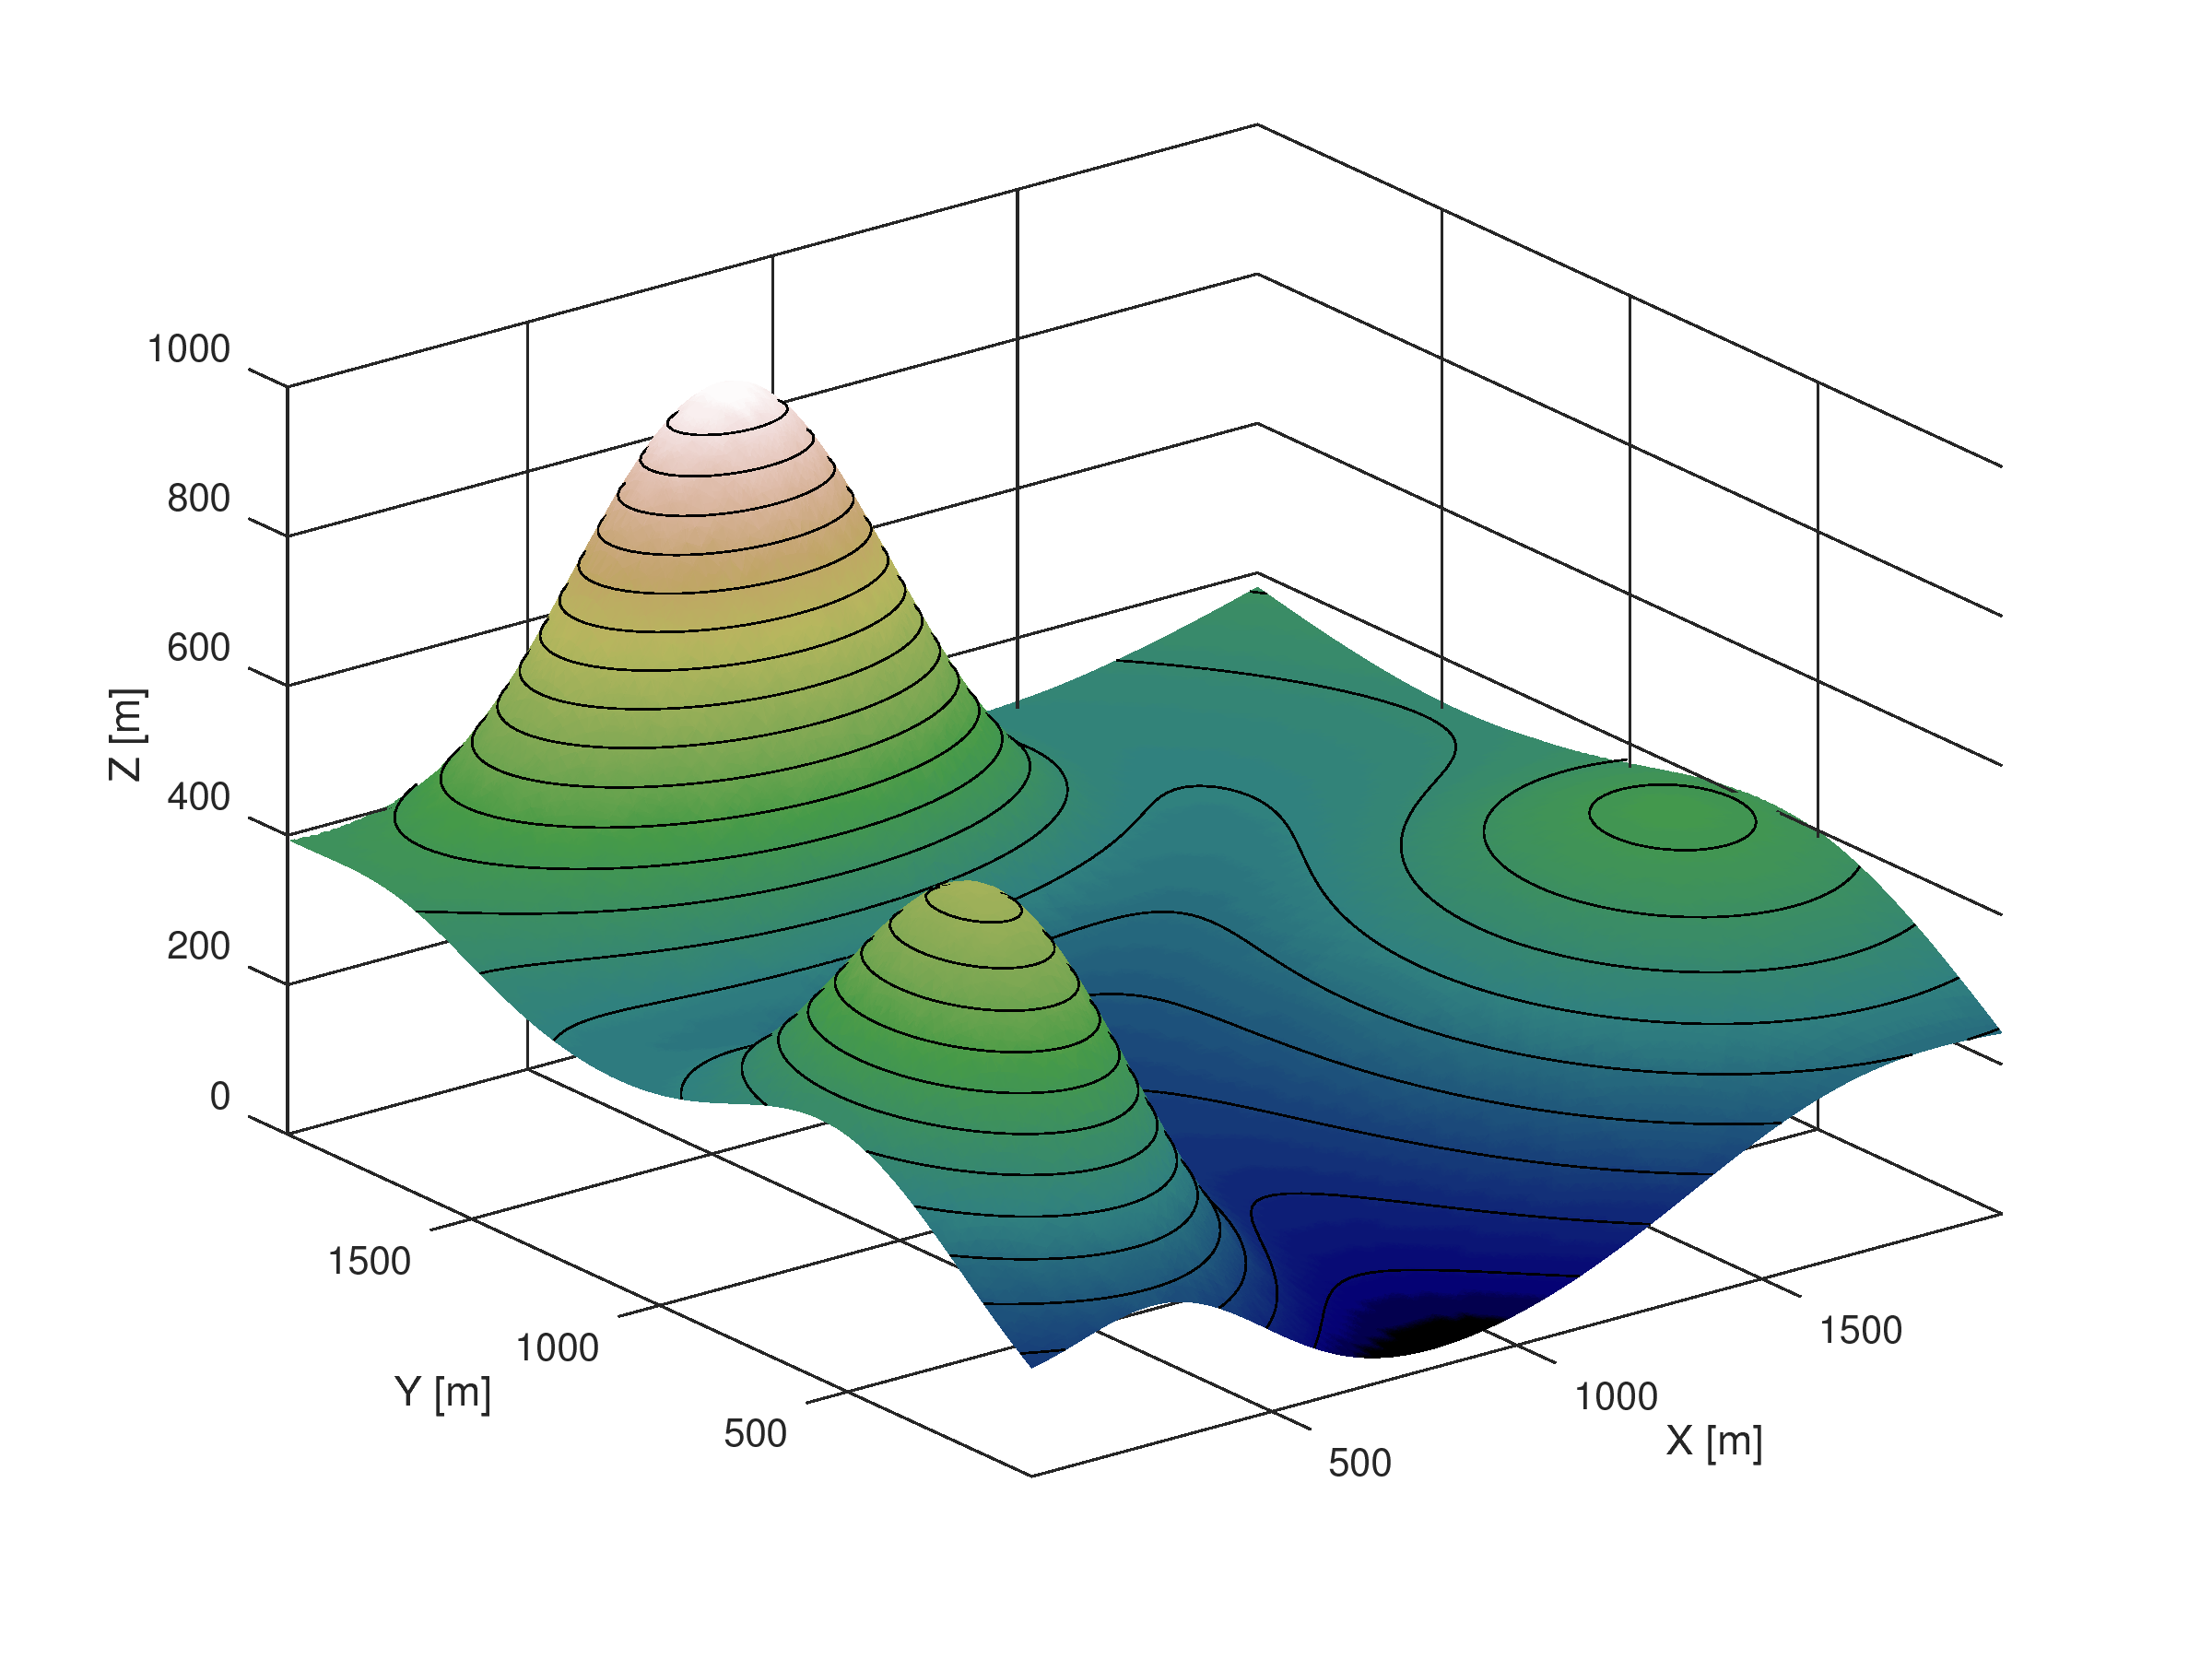
\includegraphics[width=0.7\textwidth]{Figures/topography.png}
  \caption{Synthetic topography composed of three Gaussian bumps on a sloping plane. The runoff from this domain, due to the high variability of its slope, is given by the superpositions of several waves. For the time-to-threshold flood-warning problem, this generates non-monotonous functions which make emulation challenging (see Fig.~\ref{fig:hydrograph}).}
  \label{fig:topography}
\end{figure}

%...............................................................................
\subsubsection{Setting-up the simulations}
%...............................................................................
The dataset required for building the emulator was generated by running \num{50} simulations with different combinations of the variables \emph{rain intensity} ($I$) and \emph{initial soil saturation} ($\theta_i$).
The duration of every simulation was $\approx \SI{30}{\minute}$, for a simulated time of \SI{9}{\hour}, giving a ratio real-time/simulation-time of \SI{3.3}{\minute\per\hour} simulated.
The initial soil saturation, despite being a spatially distributed variable, was kept uniform over the whole domain.
The rain intensity was kept constant and was uniformly applied over the domain, also because \citetalias{delestre_fullswof:_2017}, at this stage of development, only allows for uniformly distributed rain \autocite{laguerre_documentation_2016}.

\num{5} different initial saturations in the $[\numrange{0}{1}]$ interval and \num{10} rain intensities in the \SIrange{10}{35}{\milli\metre\per\hour} interval were taken and all their possible combinations were used as inputs for the simulations.
The rain duration was set to \SI{6}{\hour}, while a simulation duration of \SI{9}{\hour} was chosen in order to be able to observe the hydrograph recession. A time resolution of \SI{60}{\second} was used.

The parameters specific for the catchment in questions, were kept constant over all of the simulations.
These are summarized in Tab.~\ref{tab:simulations_parameters}.
The parameters marked with * are those \emph{spatially distributed}, meaning that a different value could be set for every cell.
For simplicity, a uniform catchment was used, therefore the values from the table are valid for the whole domain.
For the bottom boundary a \textit{Neumann boundary condition} was selected, allowing water to freely outflow.
Three \textit{wall boundary conditions} were set for the remaining boundaries, making sure that all of the water is lost through the bottom one.

\begin{table}[h]
  \centering
  \caption{Parameters and setting fixed for all simulations. Parameters marked with * are spatially distributed. For simplicity, these were kept uniform for the whole domain.}
  \label{tab:simulations_parameters}
  \begin{threeparttable}
    \begin{tabular}{lrl}
      \toprule
      \textbf{Parameter} & \textbf{Value} & \textbf{Units} \\
      \midrule
      Domain x-length                          &    $\num{2000}$           & \si{\meter}   \\
      Domain y-length                          &    $\num{2000}$           & \si{\meter}   \\
      Number of cells x                        &    $100$             &    \\
      Number of cells y                        &    $100$             &    \\
      Friction coefficient\tnote{*}            &    $0.03$            & \si{s.m^{-1/3}}\\
      Crust thickness\tnote{*}                 &    $1$               & \si{\meter}\\
      Crust hydraulic conductivity\tnote{*}    &    $2\cdot 10^{-6}$  & \si{\meter\per\second}\\
      Soil hydraulic conductivity\tnote{*}     &    $2\cdot 10^{-6}$  & \si{\meter\per\second}\\
      Soil suction head\tnote{*}               &    $0.09$      & \si{\meter}\\
      Soil maximum infiltration rate\tnote{*}  &    $19.8$      & \si{\milli\meter\per\hour}\\
      \bottomrule
    \end{tabular}
  \end{threeparttable}
\end{table}

%...............................................................................
\subsubsection{Extracting the datasets}
%...............................................................................
The datasets used to build the emulator was extracted from the simulation outputs in two steps.
First, the outflow hydrographs were extracted from the simulation output files, by summing up, at every time-step saved, the cell discharge along the whole domain bottom boundary. The result of this operation is a river flow time series with \num{540} observations, with a temporal resolution of 1 minute.
The same procedure was repeated for each of the 50 events, producing \num{50} different hydrographs (see Fig.~\ref{fig:hydrographs3d}).\\

Successively, the time-to-threshold $t_!$ has been computed based on the specified threshold discharge $Q_!$. 
The time-to-threshold $t_!$ paired with the corresponding rainfaill intensity and the initial soil saturation conditions formed the output-inputs sets used to construct the emulator. 

In a real situations, the threshold discharge $Q_!}$ could be the discharge at which a bridge or the embankments located on the channel are overflown. 
In order to develop the methodology, $Q_!$ was set to \SI{10}{\percent} of the $Q_{max}$ value recorded, corresponding to \SI{0.17}{\cubic\meter\per\second}.

The time at which this value is exceeded for the first time was extracted from every hydrograph and forms the dataset for the emulator.
 
By looking at one of the hydrographs extracted (Fig.~\ref{fig:hydrograph}) it can be observed that $t_!$ is a difficult quantity to predict.
In fact, depending on the $Q_!$ set, the time-to-threshold can be reached very quickly, can show a long time-lag, or not be reached at all.
Within the region defined by the $Q_!$ and the $Q'_!$ lines the hydrograph presents a plateau.
Here, a minimal variation of the threshold set can make the time-to-threshold fall towards $t_!$ or $t'_!$, hence causing a big jump in the value.
The studied quantity $t_!$ is therefore said to be \emph{discontinuous}.

\begin{figure}[h]
  \centering
  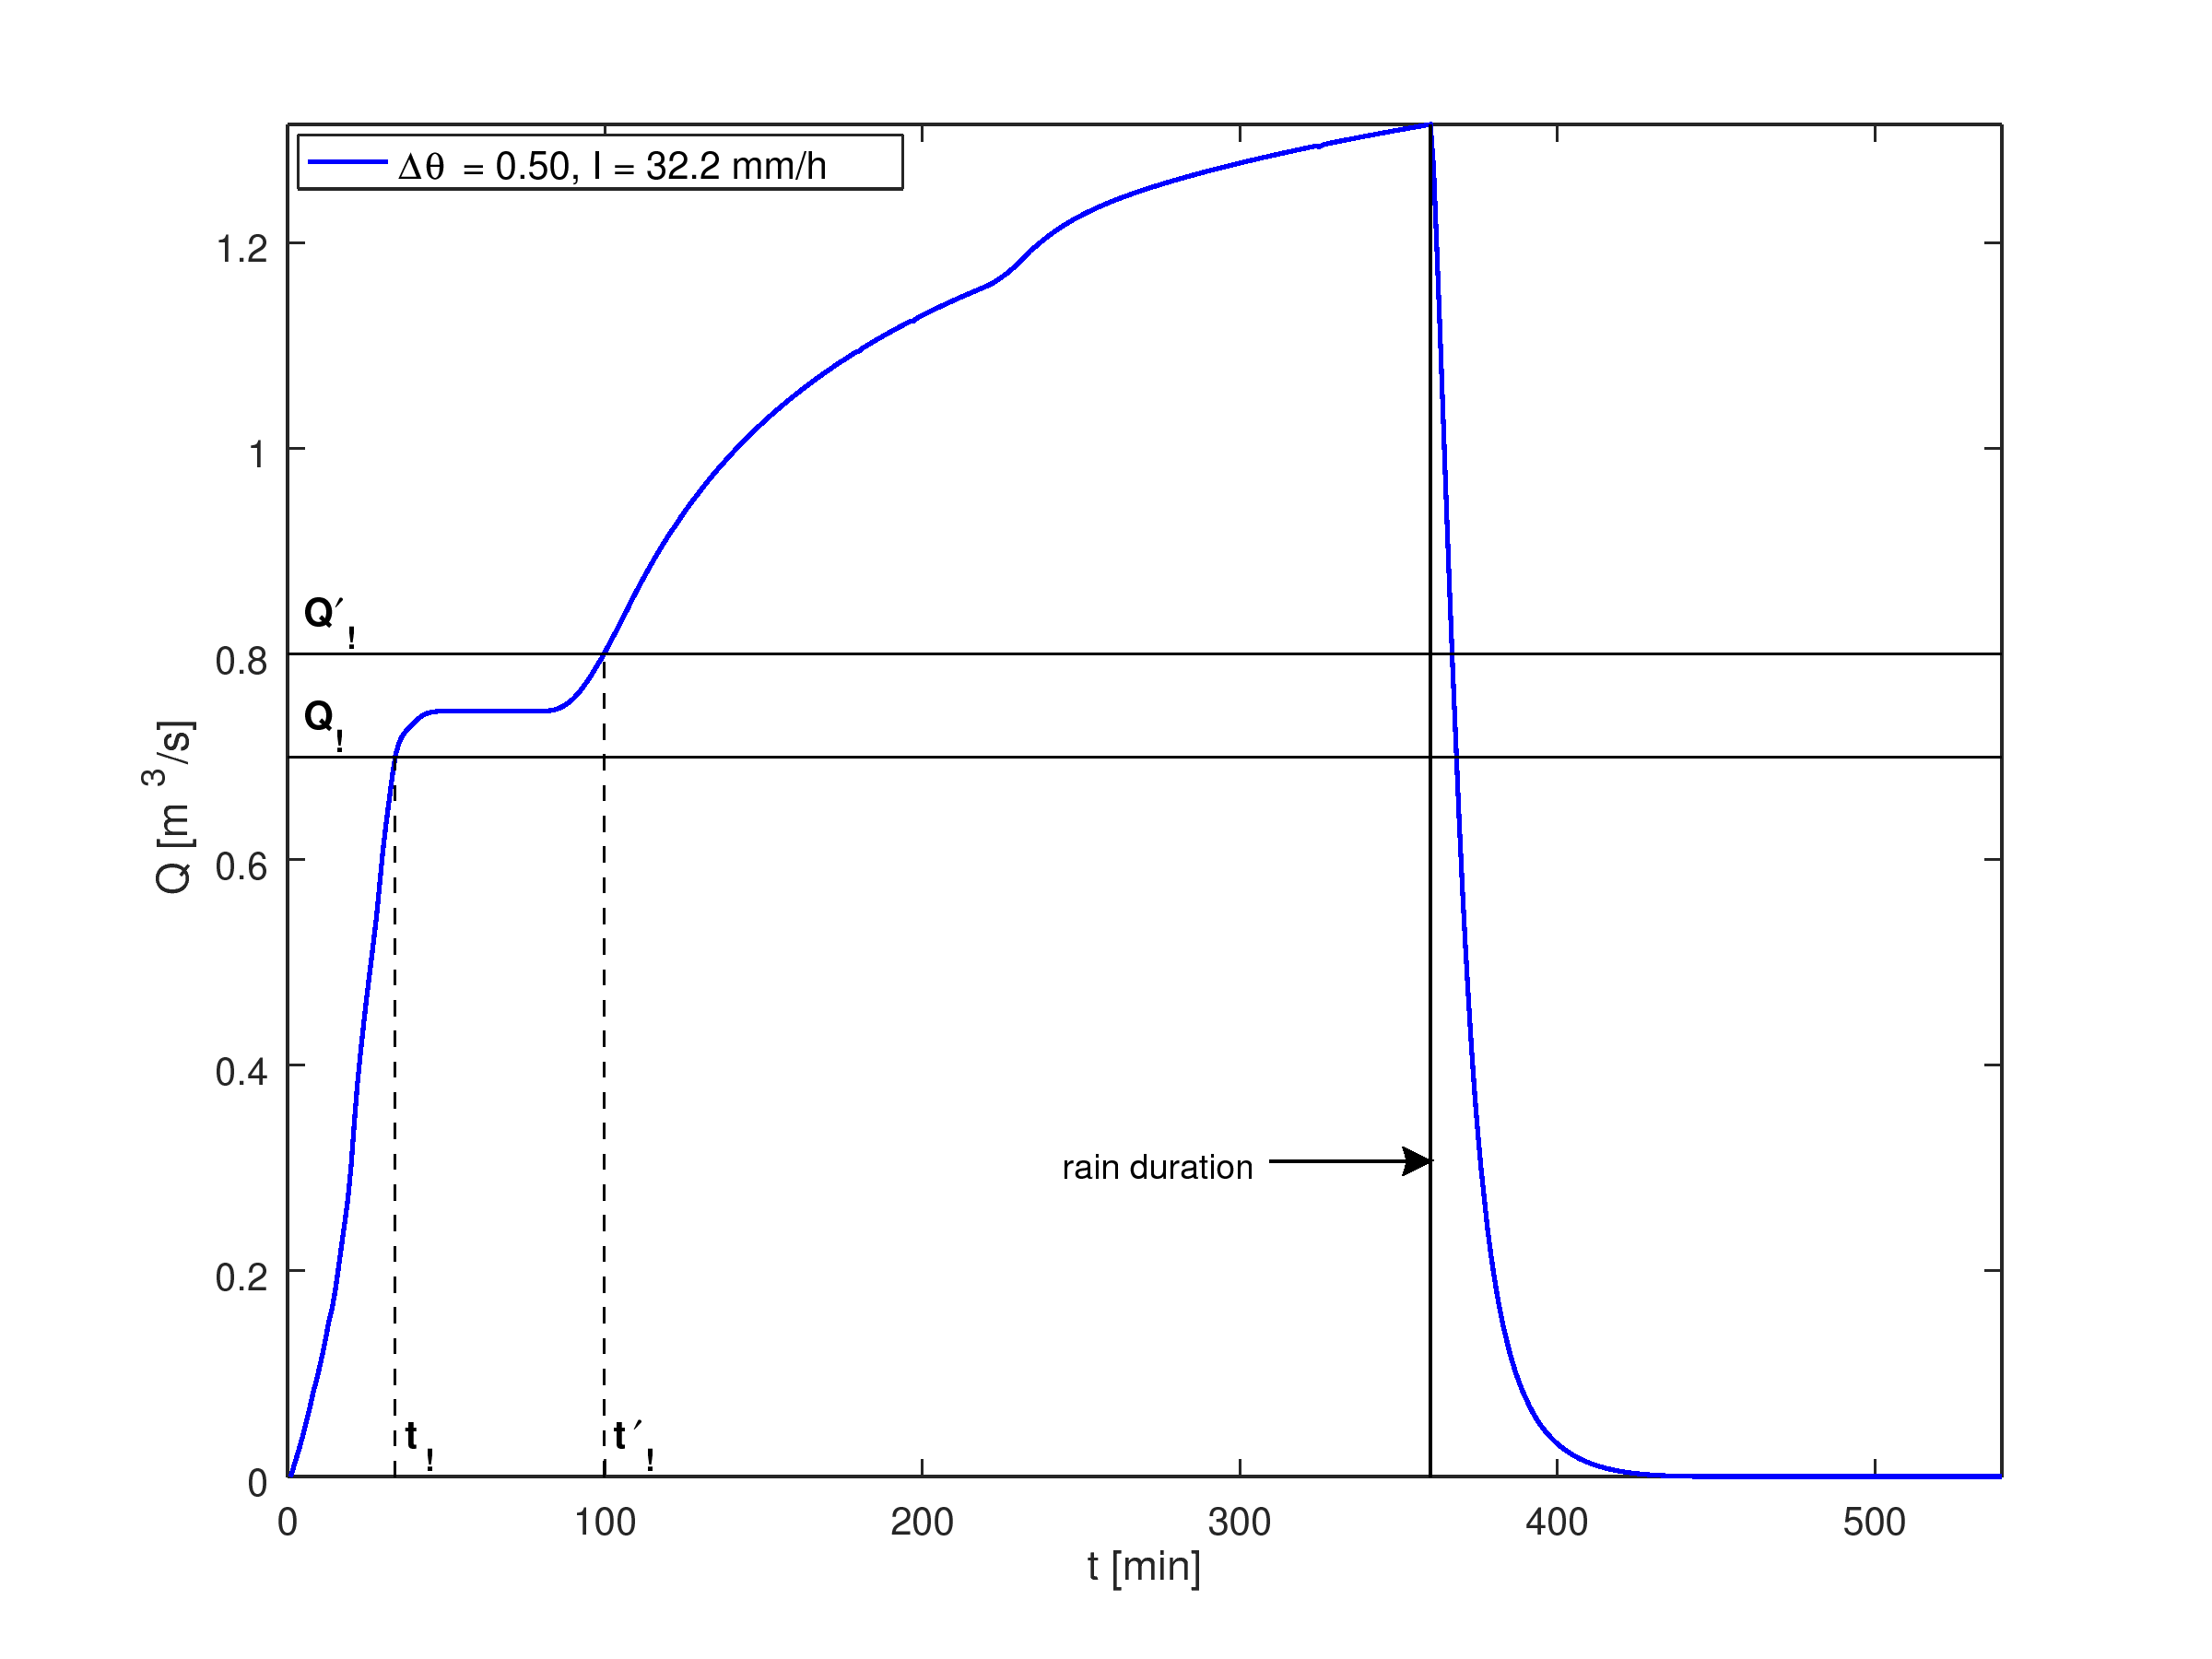
\includegraphics[width=0.7\textwidth]{Figures/hydrograph.png}
  \caption{Response hydrograph for $\theta_i = \num{0.5}$ and $I = \SI{32.2}{\milli\meter\per\hour}$. By looking at the plateau located between the $Q_!$ and $Q'_!$ lines, the discontinuity in $t_!$ can be observed. A minimal change in the threshold causes a jump in the time-to-threshold of almost an hour. This feature makes the emulation task very challenging.}
  \label{fig:hydrograph}
\end{figure}


From the same hydrographs the dataset for the classifier was also produced.
This was created by assigning the value \num{-1} to rain events not reaching the threshold and \num{1} the others.

%...............................................................................
\subsubsection{Building-up the classifier}
%...............................................................................
The classifier was built in order to ease the task of computing the time-to-threshold.
The classifier should distinguish whether a rain event is going to reach the threshold discharge or not.
Only the events classified as "reaching the threshold" are given to the emulator to compute \emph{when} this will happen.
To train the classifier we used the $\num{-1}/\num{1}$ dataset previously created.
We tested different classifier before finding a satisfying one.
To visually inspect the performance of each different classifier, we plotted the dataset in an initial soil saturation vs. rain intensity plot (Fig.~\ref{fig:classifier_rough}).
Rain events reaching the threshold are marked with red circles, while rain events not reaching it with green ones.
We built the classifier using GP---this with the help of the package \citetalias{rasmussen_gaussian_2010} for \citetalias{octave_community_gnu_2018}.
The data seemed to be linearly separable, therefore we used the "meanLinear" mean function.
We combined this with different covariance functions and trained the models with the "minimize" function, by using a "likLogistic" likelihood function and the Expectation Propagation (EP) as inference method.
The use of the "meanLinear" mean function with a "covConst" covariance functions produced good results: the dataset could be linearly separated (see Fig~\ref{fig:classifier_rough} in the Appendix).
However, infinite different curves could define the frontier between events reaching and not reaching the threshold.
After we obtained this first border we added new data points in its proximity by running new simulations.
With these we followed the exact same procedure explained above.
We added these new observations to the classifier's training dataset and plotted them as triangles, in order to distinguish them from the previous ones.
The new data points suggested that the boundary is actually not linear; it has a curvy shape instead.
We therefore chose a curvy mean function and combined it with various covariance functions.
After training many models an optimal set of mean, covariance and likelihood functions combined with the use of EP inference method could be found. These results can be found under Sec.~\ref{sec:classifier}.
One point could not be separated with any set of functions tried.

%...............................................................................
\subsubsection{Building-up the emulator}
%...............................................................................
The procedure we used to build the time-to-threshold emulator is very similar to the one used for the classifier.
We plotted the \num{50}-points dataset as red dots in a 3D graph, where the x and y axis are given by the rain intensity $I$ and the initial soil saturation $\theta_i$ respectively.
The z-axis shows the response of every rain event, namely the time-to-threshold, which we previously extracted.
We created a $(I, \theta_i)$ grid where to evaluate the emulator:\\

\inputminted[
  fontsize=\footnotesize,
  firstline=30,
  lastline=42,
  numbersep=2pt,
  gobble=0,
  frame=none,
  bgcolor=light-gray,
  framesep=10mm
]{octave}{code.m}\\

\noindent Then we performed a GP regression on the training dataset using the \citetalias{rasmussen_gaussian_2010} package.
As for the classifier, we tested different combinations of mean, covariance and likelihood functions with arbitrary initial hyperparameters values.
As an inference method we used the "infExact" one.
We minimized the negative log marginal likelihood with the "minimize" function and with this we obtained the optimized values for the hyperparameters.
We then evaluated the obtained model on the $(I, \theta_i)$ evaluation grid which we previously created.
Since it was sometimes difficult to establish which GP was performing better we produced a new dataset, the \emph{test dataset}.
We created the test dataset the same way we generated the training one, but using different $(I, \theta_i)$ values.
The values of $I$ and $\theta_i$ used can be produced with the code found in Sec.~\ref{sec:test_dataset} of the Appendix.
The test dataset has \num{36} points given by all possible combinations of these values.
We then added the test dataset to the plot and used it to evaluate the performance of the models far from the observations used for the training.
With these points guiding us we found the model producing the best results.
The \emph{test dataset} was then included in the dataset used for training, in order to further improve the emulator's performance.
Finally, we originated a \nth{3} dataset, the \emph{validation dataset}.
This is constituted by \num{6} points sparse in the inputs space.
The values of the $(I, \theta_i)$ pairs composing this dataset can be found in Tab.~\ref{tab:validation_dataset} of the Appendix.
These observations constitute an unbiased dataset, since it was never shown to the model.
We evaluated the performance of our model on both test and validation dataset by computing the MAE and the RMSE.


%-------------------------------------------------------------------------------
\subsection{Results}
%-------------------------------------------------------------------------------
%...............................................................................
\subsubsection{Simulations}\label{sec:simulations_results}
%...............................................................................

\begin{figure}[h]
  \centering
  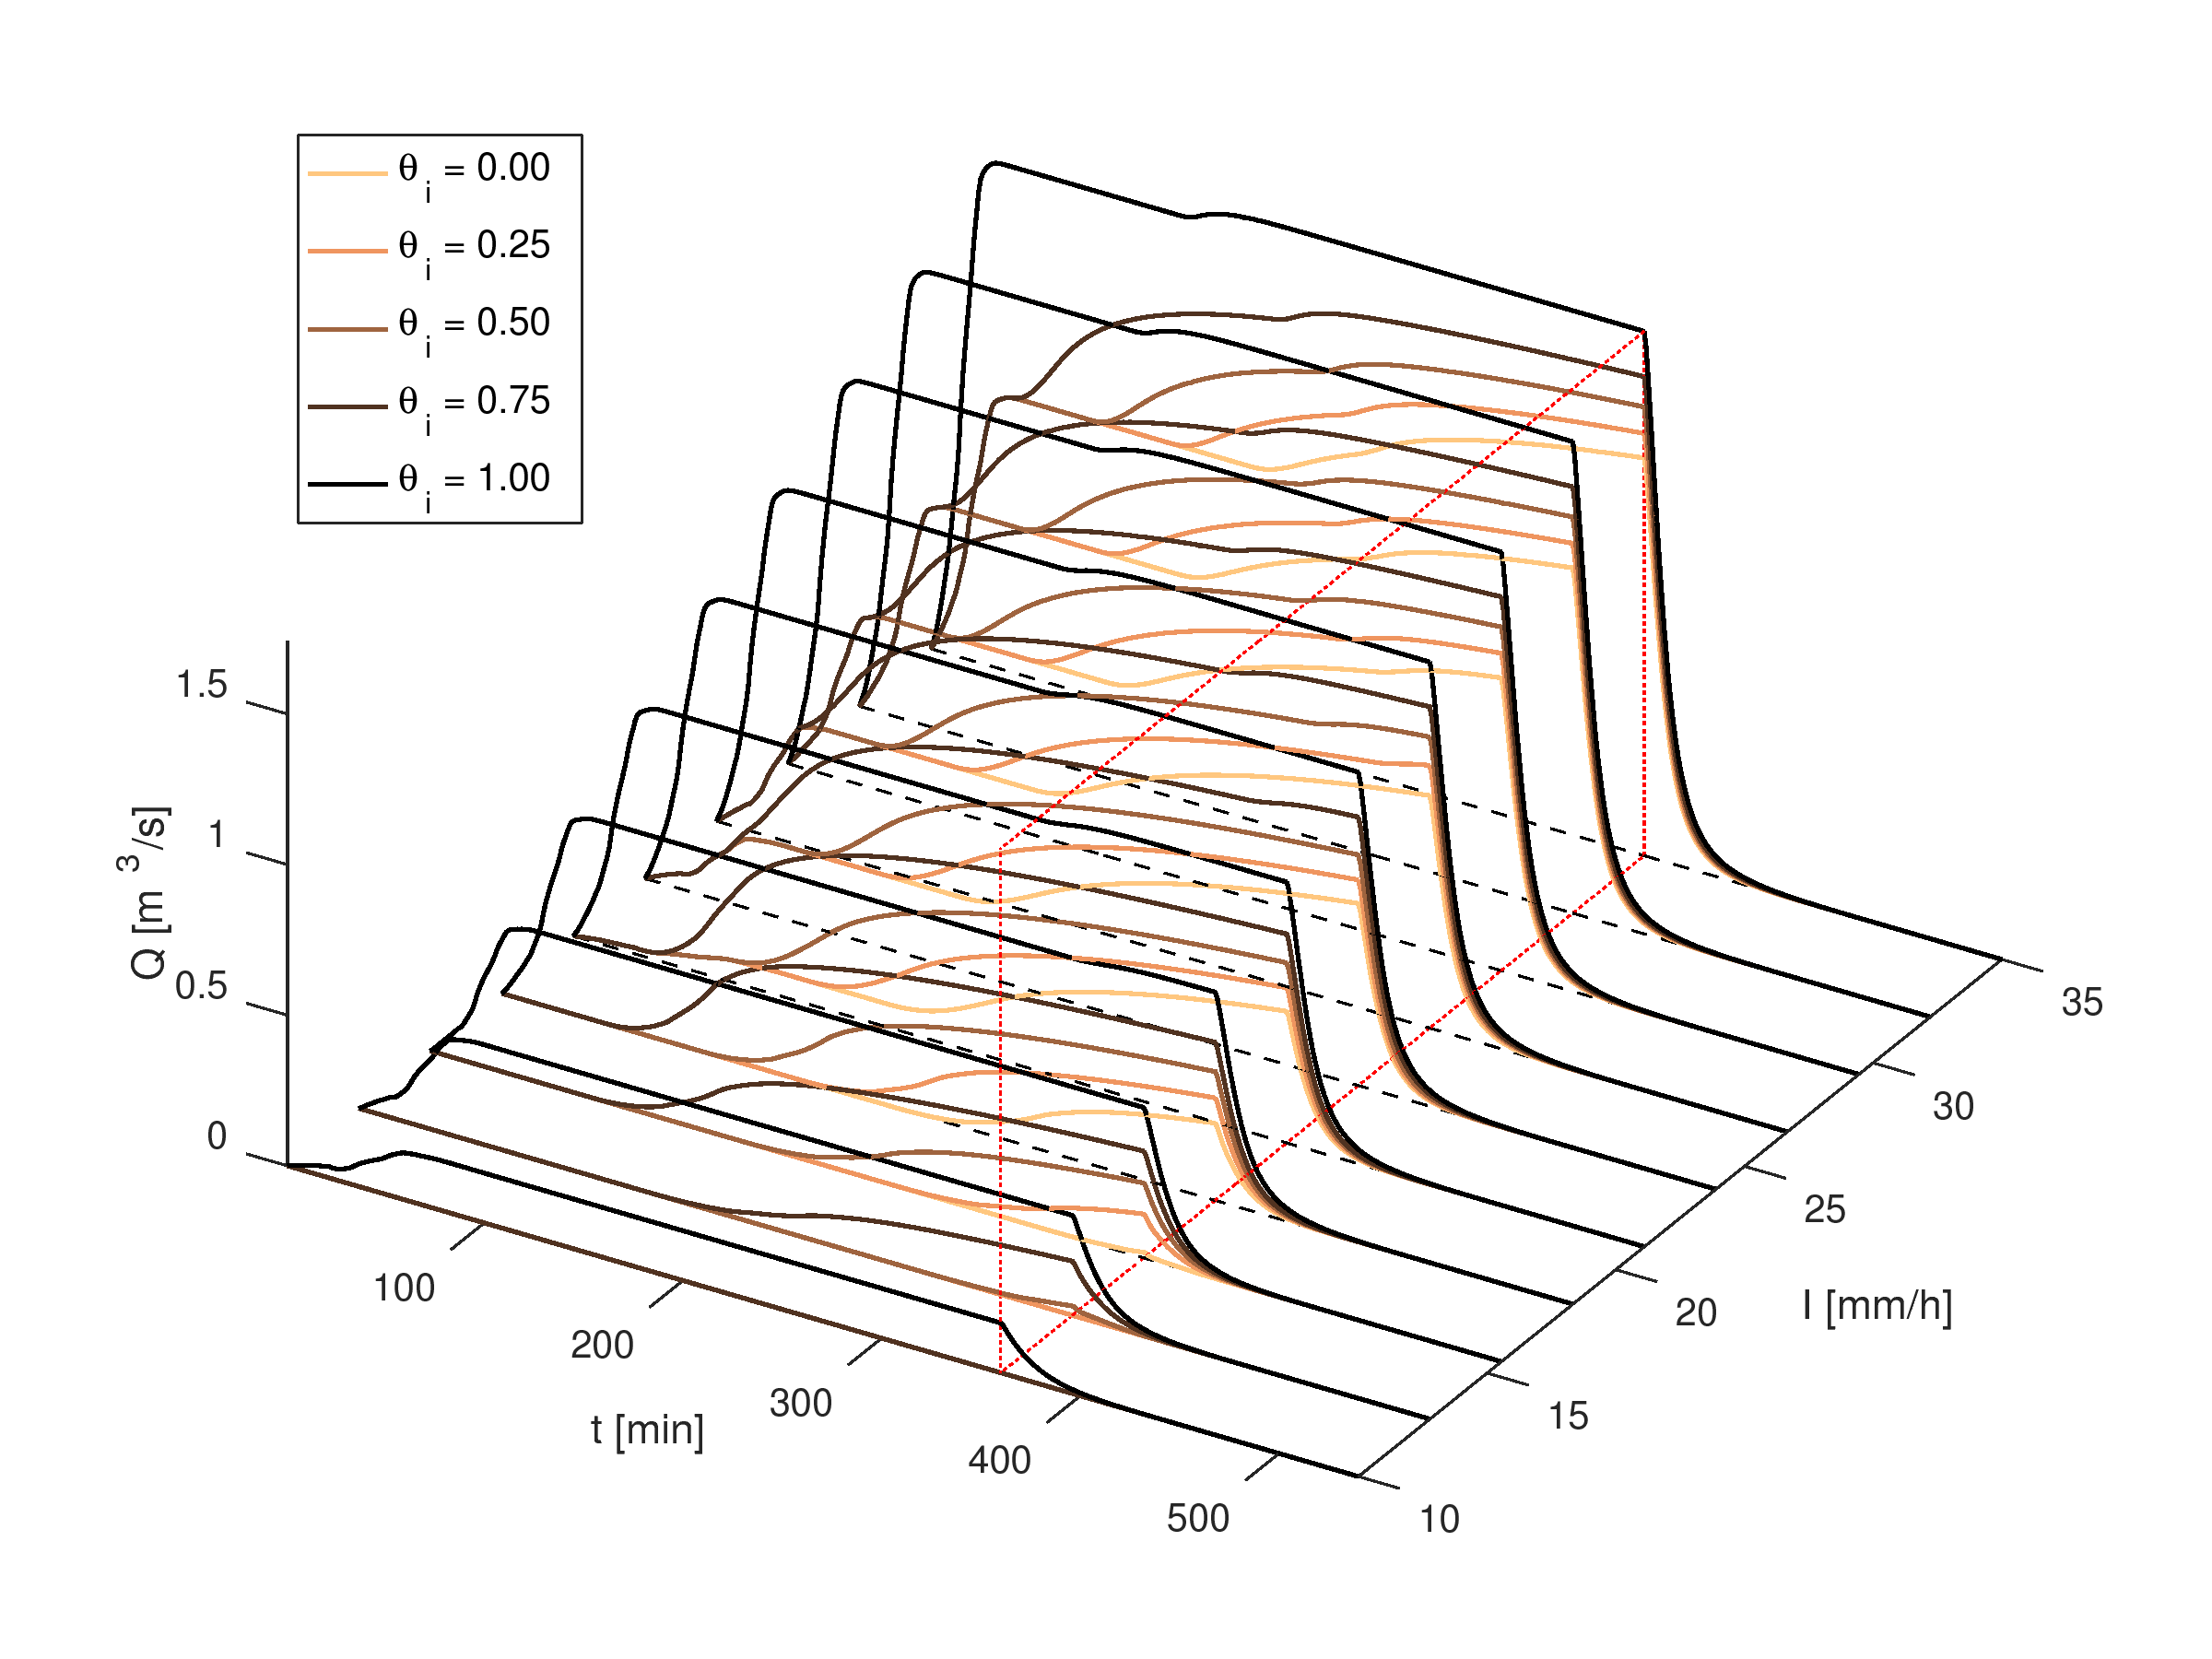
\includegraphics[width=0.75\textwidth]{Figures/hydrographs3d.png}
  \caption{Response hydrographs for the \num{50} simulations at the catchment outlet. The red frame shows the end of the rain event. Depth-dimension shows the \emph{rain intensity} variable, while the \emph{initial saturation} variable is rendered by the colormap. It can be observed, that shape and magnitude of the response vary considerably from one simulation to the other.}
  \label{fig:hydrographs3d}
\end{figure}


Fig.~\ref{fig:hydrographs3d} shows the \num{50} obtained hydrographs.
Here many interesting features can be observed.
It can be seen that experiments run with the two lowest rain intensities and low initial soil saturation generated no discharge.
In the second place, simulations run with $\theta_i = \num{1}$ always reached their peak discharge, and this happened quite quickly.
Some of these show a second smaller increase after the first quick rising limb.
This is even more accentuated in the simulations were the soil was initially not saturated.
We can explain this effect as the mapping of the topography configuration to the response hydrographs.
The topography used presents zones with very steep slopes and others with very flat ones, causing different flow velocities.
This results in water at the same distance from the outlet arriving with different travel times.
When the water from the inclines has reached the outlet, that coming from flat areas is still traveling downstream.
After a given lapse of time this water reaches the outlet as well, giving rise to the bumps visible in the hydrographs.\\

%...............................................................................
\subsubsection{The classifier}\label{sec:classifier}
%...............................................................................
% * Classifier:
%   * show final values of hyperparameters

Fig.~\ref{fig:classifier} displays the results of the classification task.
Green data points correspond to rain events which did not exceed the threshold, while the red ones to those which did.
Circles show the initial dataset (training dataset), whereas triangles indicate the dataset which was added in a second time.
According to the classifier every $(I, \theta_i)$ pair chosen in the yellow region will cause the exceeding of $Q_!$.
The classifier could correctly classify all but one points given.
The triangle located at $(I, \theta_i) = (14.7, 0.45)$ is found within the yellow region although its color is green.

\begin{figure}[h]
  \centering
  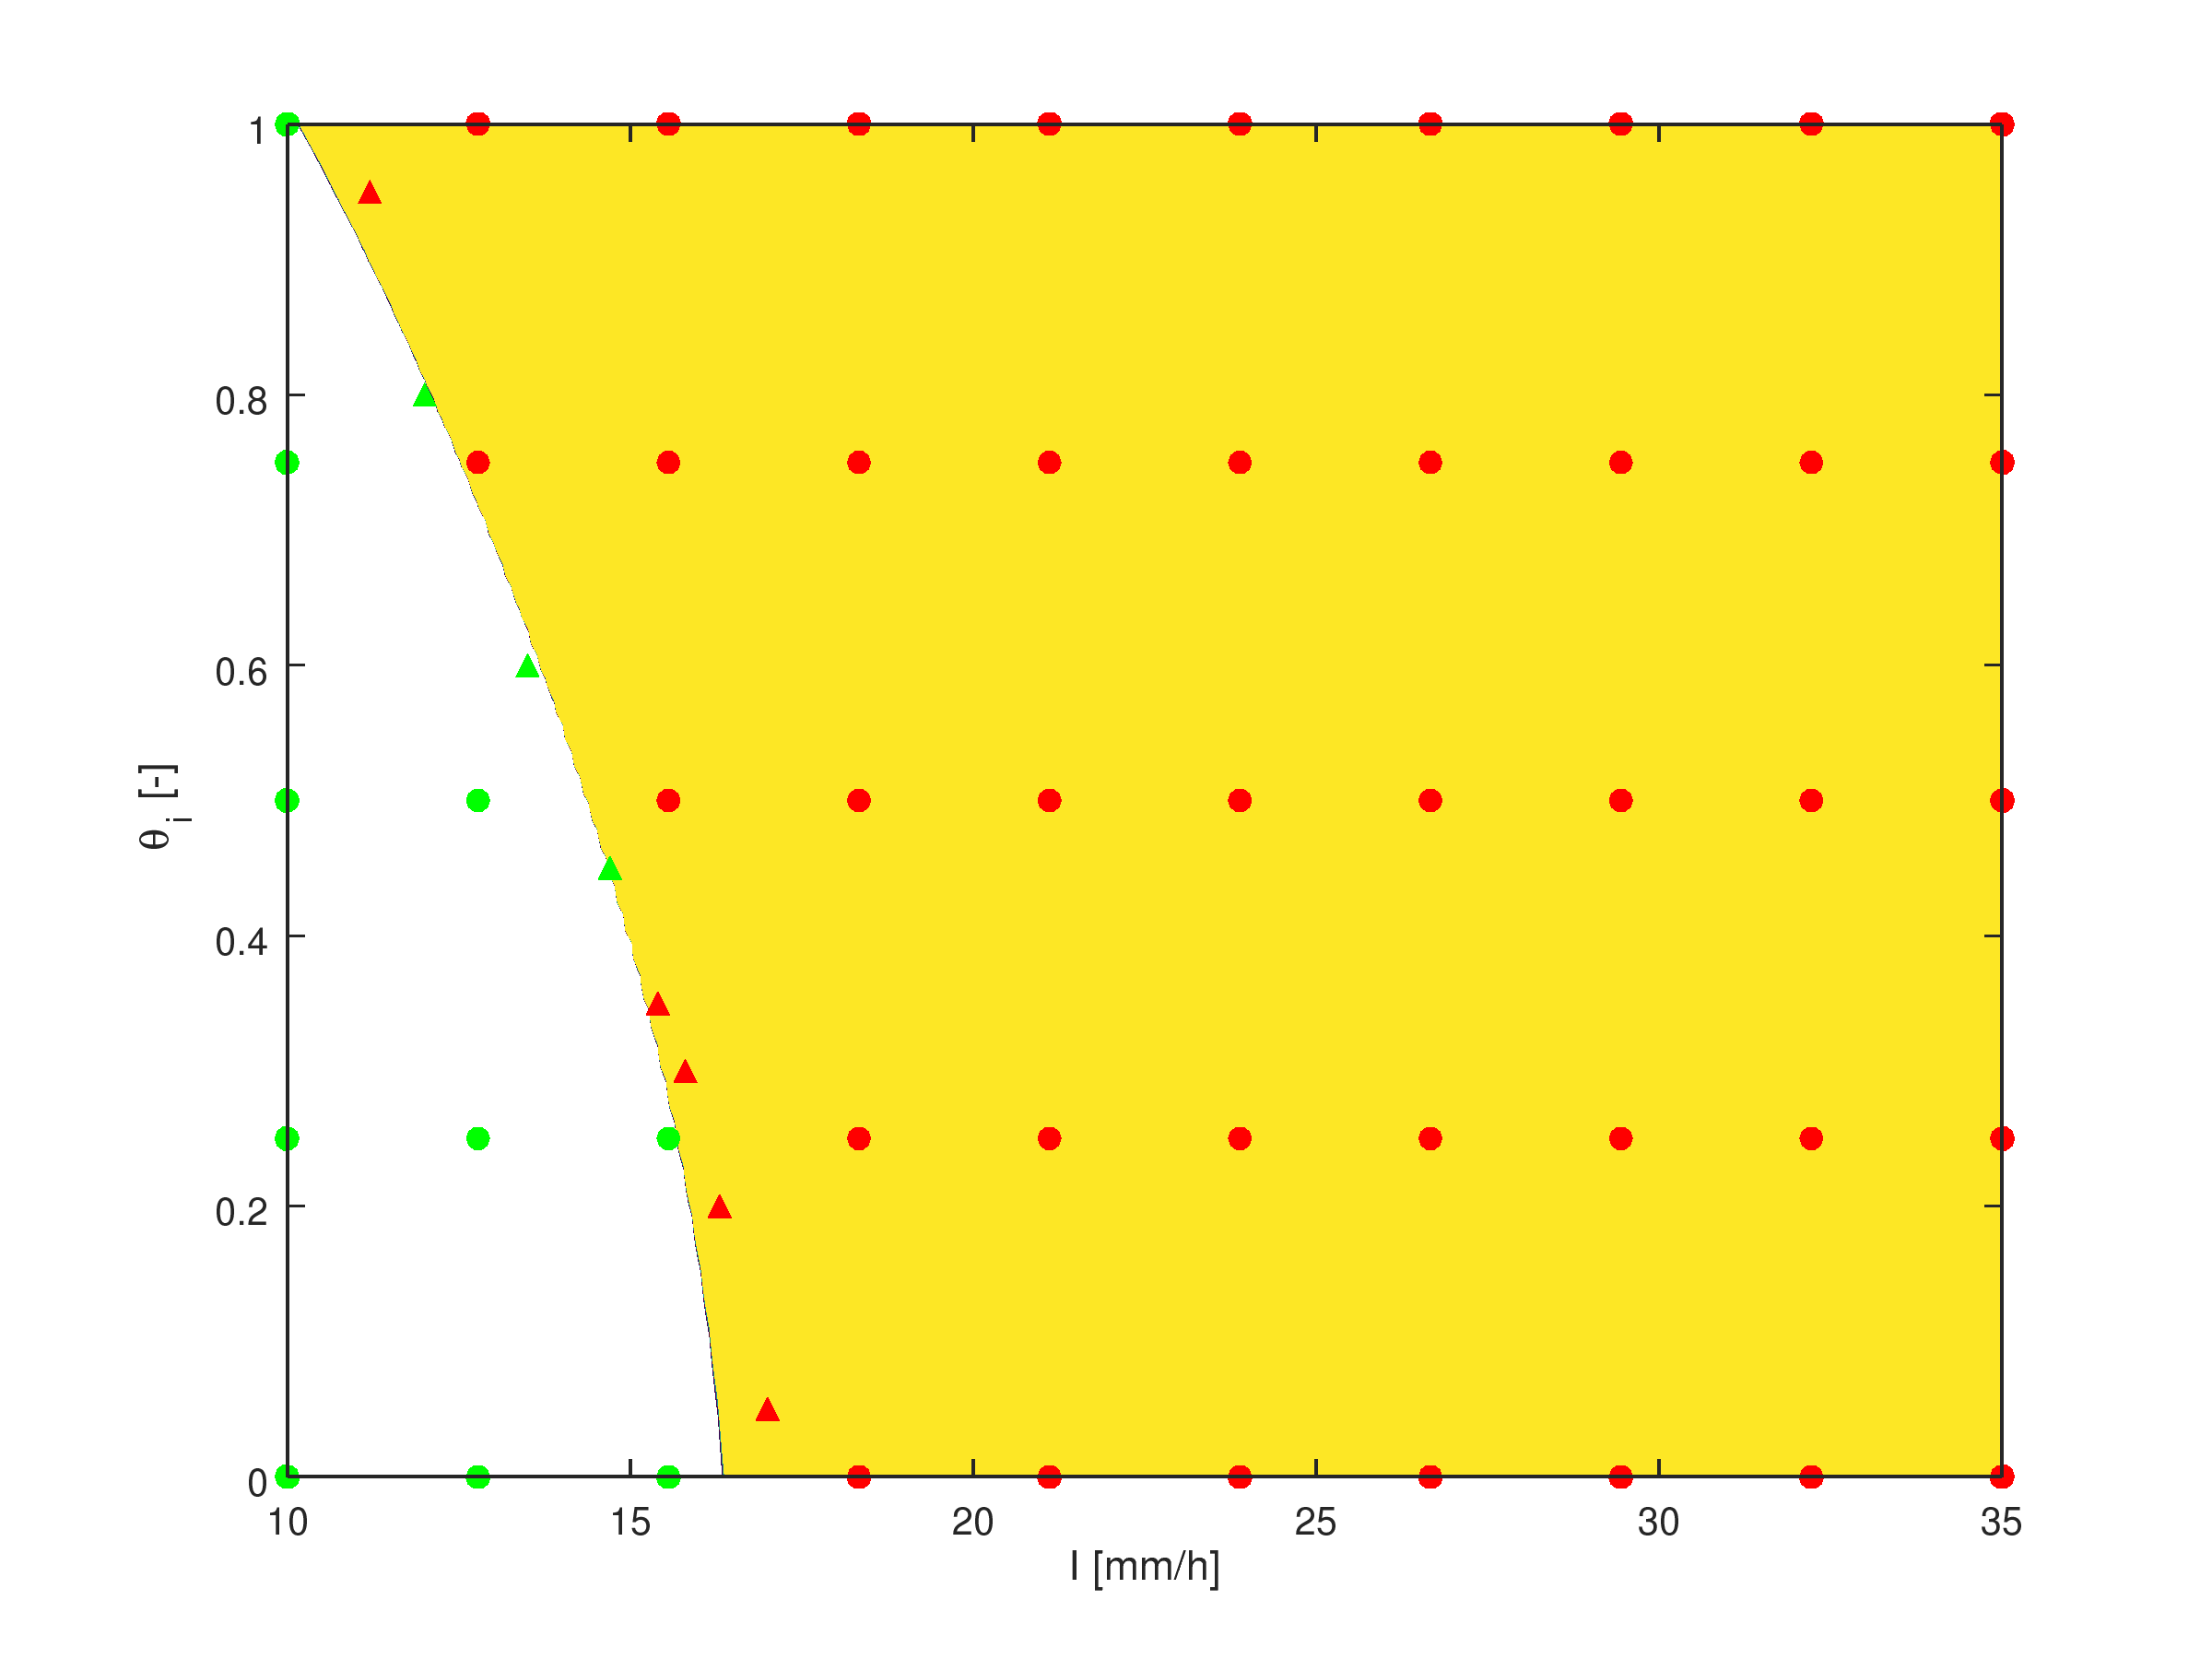
\includegraphics[width=0.7\textwidth]{Figures/classifier.png}
  \caption{Classifier: the circles represent the first training dataset, while the triangles the second one. In red all events exceeding the threshold, in green all those which did not. Events in the yellow region are the ones classified as "exceeding the threshold", for which the time-to-threshold has to be estimated.}
  \label{fig:classifier}
\end{figure}

The portion of code here below shows the mean, covariance and likelihood functions set which produced the best results.
The arbitrary hyperparameters values set here were then optimized with the "minimize" function.
The final values can be found under Sec.~\ref{sec:classifier_hyperparameters} of the Appendix.\\

\inputminted[
  fontsize=\footnotesize,
  firstline=14,
  lastline=22,
  numbersep=2pt,
  gobble=0,
  frame=none,
  bgcolor=light-gray,
  framesep=10mm
]{octave}{code.m}


%...............................................................................
\subsubsection{The emulator}
%...............................................................................
\begin{figure}[h]
  \centering
  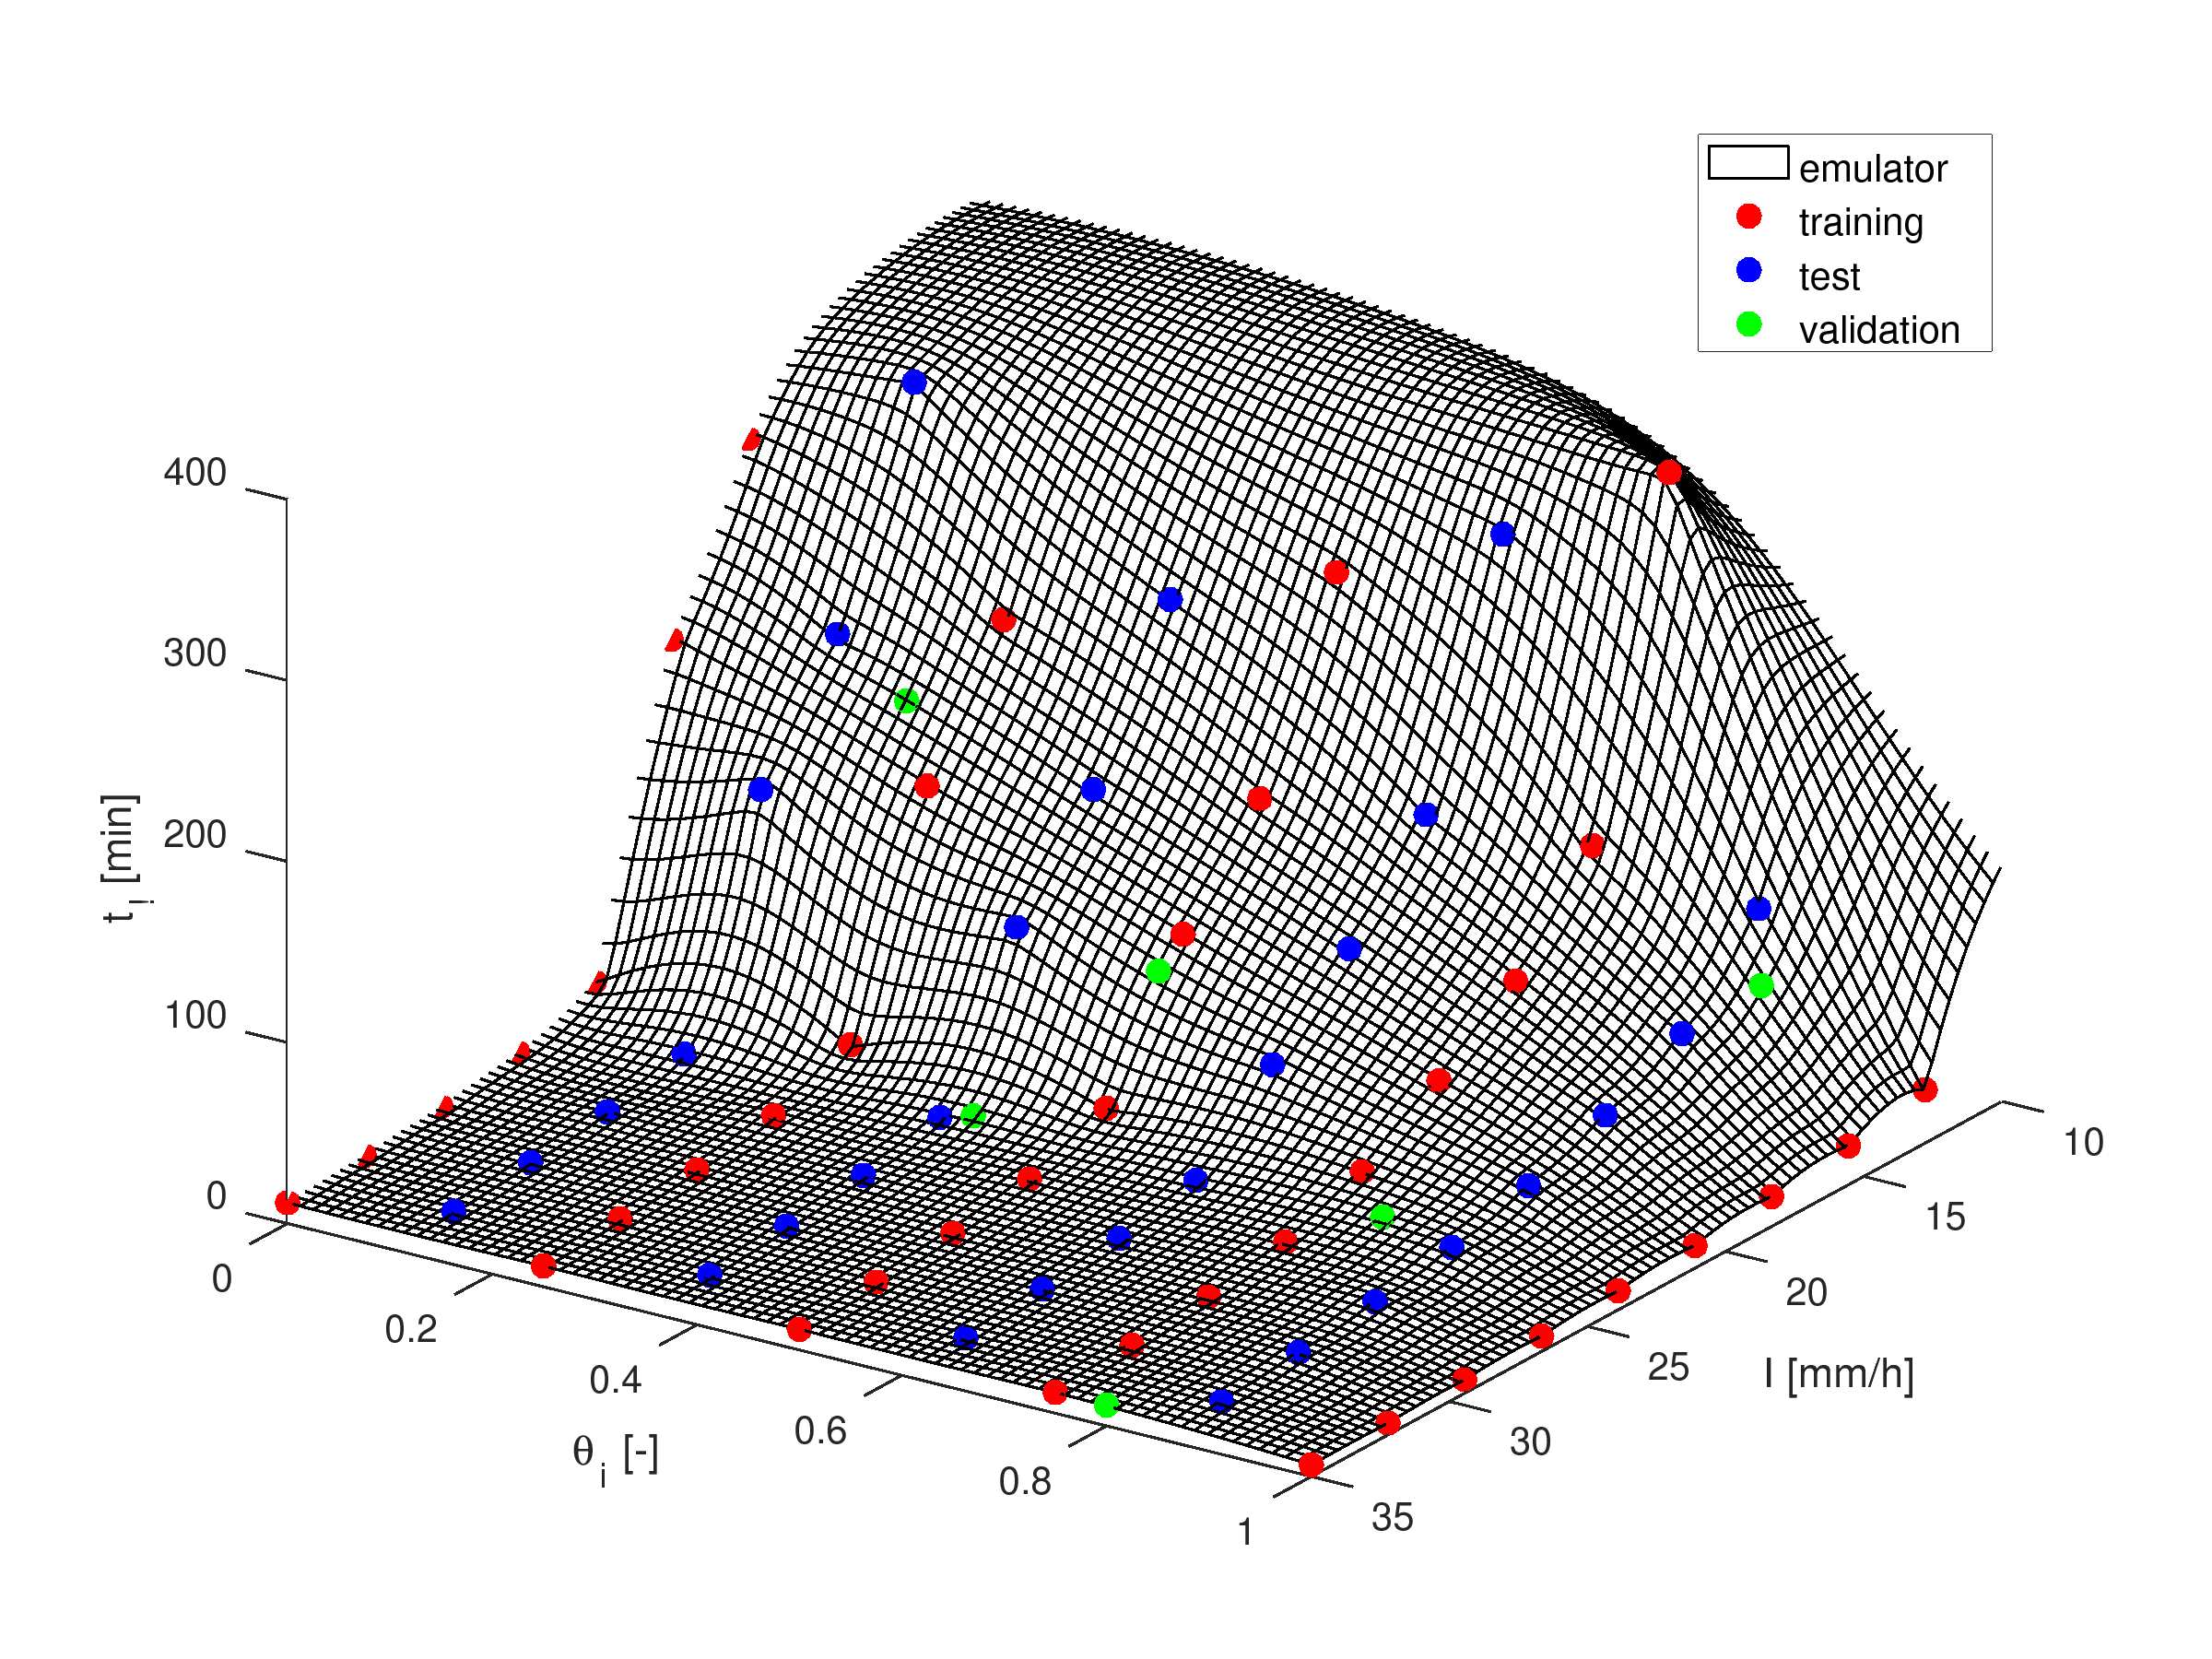
\includegraphics[width=0.8\textwidth]{Figures/emulator.png}
  \caption{Time-to-threshold emulator: training (red), test (blue) and validation (green) datasets and the emulator (mesh) predicting the time-to-threshold ($t_!$) in regions where there are no observations. The emulator interpolates all of the training points (red and blue ones). The extrapolation far outside the observations boundaries are meaningless. These are already discarded by the classifier.}
  \label{fig:emulator}
\end{figure}

The time-to-threshold emulator is shown in Fig.~\ref{fig:emulator}.
The x and y axis indicate the value of the inputs---rain intensity and soil saturations---while the corresponding response is given on the z-axis.
The circles represent the datasets used for training (red), testing (blue) and validating (green).
The emulator is given by the black mesh and is the result of the evaluation of the optimized GP at the \num{6400} evaluation points.
The set of mean, covariance and likelihood functions with which the emulator was obtained were:\\

\inputminted[
  fontsize=\footnotesize,
  firstline=76,
  lastline=84,
  numbersep=2pt,
  gobble=0,
  frame=none,
  bgcolor=light-gray,
  framesep=10mm
]{octave}{code.m}\\

\noindent The optimized values of the GP hyperparameters can be found under Sec.~\ref{sec:emulator_hyperparameters} in the Appendix.\\

The performance of the emulator was assessed by computing MAE and RMSE of the validation and test datasets. These provides an estimation of the out-of-sample error.
These results are summarized in Tab.~\ref{tab:emulator_performance}.




\begin{table}[h]
  \centering
  \caption{Emulator performance on \emph{test} and \emph{validation} datasets. The test dataset was also used for model interpolation, for this reason it shows "no error".}
  \label{tab:emulator_performance}
  \begin{tabular}{lcc}
    \toprule
     & \textbf{MAE [\si{\minute}, \si{\percent}]} & \textbf{RMSE [\si{\minute}]} \\
    \midrule
    \textbf{test}       & $8.0\cdot 10^{-5},\,5.2\cdot 10^{-5}$ & $2.3\cdot 10^{-5}$\\
    \textbf{validation} & $6.0,\,5.9$ & $4.0$\\
    \bottomrule
  \end{tabular}
\end{table}

The emulator's speedup factor was also computed.
The evaluation of the emulator at one point lasts in average \SI{0.012}{\s}, whereas running a simulation takes approximately \SI{30}{\minute}.
This represents a \emph{speedup} of \textbf{\num{150000}} $\bm{\times}$.

%-------------------------------------------------------------------------------
\subsection{Discussion}
%-------------------------------------------------------------------------------
% * emulator should never underestimate danger -> we want to avoid it
%   absolutely)
% * discuss point misclassified
% * discuss influence of time resolution
% * discuss emulator's speedup
% * if a real system is built -> UQ very important!!


Crucial for an early flood warning system, is to avoid underestimating the danger.
This means, the time to thresholds predicted by our emulator are allowed to be shorter than the real ones, but not longer.
Our emulation-based early flood warning system is the sum of the \emph{classifier} and the \emph{emulator}.
Information about the rain event are passed to the classifier (forecasted rain intensity and estimated soil saturation of the catchment).
The classifier accomplishes the first task: assessing if the rain event will reach the given threshold or not.
Under Sec.~\ref{sec:classifier} we saw that the classifier proposed for this catchment and the chosen $Q_!$ fails to classify one point.
In this case the classifiers assigns "reaching threshold" to a point which is actually not reaching it.
In such a scenario, as the one imagined, this error would be quite serious but not dangerous: temporary flood control measures would be prepared, the population would be warned but at the end no flooding would occur.
This would cost money but nobody would be armed.
The misclassified point is a training point.
This means that a better classifier should be found, by further varying the GP used for the classification.
Once a classifier correctly separating all training points is found, its performance should be evaluated.
For this a new dataset, with points close to the newly determined frontier should be created.
The classifier should then be tested with this dataset.
Its performance is given by the ratio "correctly classified" over "total data points".
If this outcome was satisfactory, then we could keep the classifier obtained.
If not we would add the new dataset to the training dataset, retrain the classifier and retest it on a further dataset that has to be produced.
This procedure should be repeated until satisfactory results are reached.
Unfortunately, this could not be done to a further extent due to lack of time.
For application to a real case it would be crucial to train a very good classifier.
From this depends if the authorities in charge would take actions or if nothing at all is done in case of a potential flooding.
Dramatical consequences could happen, if based on the classifier no action is taken but the threshold is reached.\\

The emulator, representing the second step of the early flood warning system, even if to a minor extent, should also never underestimate the risk.
The danger linked with underestimating how fast $Q_!$ is reached is somehow a bit smaller: measures are being taken when unexpectedly the flood arrives---but still to consider.
The MAE obtained on the validation datasets is \SI{6.0}{\minute}, \SI{5.9}{\percent} respectively.
In this case, it was predicted that an event reaching the threshold after \SI{101.5}{\minute} would have reached it after \SI{95.5}{\minute} and that another one reaching it after \SI{192.5}{\minute} would have reached it after \SI{198.0}{\minute} (cf. Tab.~\ref{tab:validation_performance} in the Appendix).
Those are the validation data points where the error was maximum.
In the second case we are underestimating the error, but this by a fairly small amount of time.
The absolute RMSE, \SI{4.0}{\minute} is quite close to the MAE, the MAE being just \SI{2}{\minute} higher than the RMSE.
This seem to indicate that the distribution of the error is quite narrow and that the model typically produces prediction errors of about $\approx \SI{5}{\minute}$.

The time resolution used for the simulation was \SI{1}{\minute}.
For this reason, validation errors which magnitude is smaller than this value cannot be considered as such, since at the simulation level the time-to-threshold uncertainty is already of the order of \SI{1}{\minute}.
The time resolution can have also played a role in the shape of the emulator's surface.
The mesh shows regions where the surface is less smooth, in particular in proximity of some test data points, where small peaks can be observed.
These are due to the interpolation done by the GP.
In order to interpolate the points the surface grows more than what could seem "natural".
We need to remember that the location of these points on the $t_!$ has an uncertainty of \SI{1}{\minute}, due to the resolution chosen.
This means that each point could actually be shifted up or down by \SI{1}{\minute}, which could produce these "unnatural" peaks observed.\\

Although the global performance seems to be good, particular attention have to be paid.
These prediction errors are found when no uncertainty on the parameters is considered.
When using this flood warning system in a real case the parameters values passed to the emulator, forecasted rain intensity and initial soil saturation in particular, can be very uncertain.
For this an uncertainty quantification should be carried out, in order to know which influence would have the estimated input uncertainty on the output.
The same has to be done when using a detailed simulator.
The emulator here proves to be very useful, since uncertainty quantification requires several model runs.
With the speedup obtained with our emulator, this task is \textbf{\num{150000}} more efficient.

This same speedup also offers the possibility of adapting our predictions in near-real time.
Outputs from our emulator can be reevaluated during the happening of the rain event if changing conditions are detected.
In particular, uncertainty on the rain intensity decreases for short term forecasting, making prediction of our emulator more certain the nearer in time we are to the occurrence of the rain event.




